%
% Template Laporan Skripsi/Thesis 
%
% @author  Andreas Febrian, Lia Sadita 
% @version 1.03
%
% Dokumen ini dibuat berdasarkan standar IEEE dalam membuat class untuk 
% LaTeX dan konfigurasi LaTeX yang digunakan Fahrurrozi Rahman ketika 
% membuat laporan skripsi. Konfigurasi yang lama telah disesuaikan dengan 
% aturan penulisan thesis yang dikeluarkan UI pada tahun 2008.
%

%
% Tipe dokumen adalah report dengan satu kolom. 
%
\documentclass[12pt, a4paper, onecolumn, oneside, final]{report}

% Load konfigurasi LaTeX untuk tipe laporan thesis
\usepackage{uithesis}
\usepackage{listings}
\renewcommand\lstlistingname{\hfill Daftar Kode \hfill}
\renewcommand\lstlistlistingname{\hfill Daftar Kode \hfill}
\lstdefinestyle{customc}{
	belowcaptionskip=1\baselineskip,
	breaklines=true,
	frame=L,
	xleftmargin=\parindent,
	language=C,
	showstringspaces=false,
	basicstyle=\footnotesize\ttfamily,
	keywordstyle=\bfseries\color{green!40!black},
	commentstyle=\itshape\color{purple!40!black},
	identifierstyle=\color{blue},
	stringstyle=\color{orange},
}

\lstdefinestyle{customasm}{
	belowcaptionskip=1\baselineskip,
	frame=L,
	xleftmargin=\parindent,
	language=[x86masm]Assembler,
	basicstyle=\footnotesize\ttfamily,
	commentstyle=\itshape\color{purple!40!black},
}

\lstset{escapechar=@,style=customc}

% Load konfigurasi khusus untuk laporan yang sedang dibuat
%-----------------------------------------------------------------------------%
% Informasi Mengenai Dokumen
%-----------------------------------------------------------------------------%
% 
% Judul laporan. 
\var{\judul}{Analisis Kinerja Container untuk Virtual Screening Tanaman Obat Asli Indonesia dengan Autodock dan Autodock Vina}
% 
% Tulis kembali judul laporan, kali ini akan diubah menjadi huruf kapital
\Var{\Judul}{Analisis Kinerja Container untuk Virtual Screening Tanaman Obat Asli Indonesia dengan Autodock dan Autodock Vina}
% 
% Tulis kembali judul laporan namun dengan bahasa Ingris
\var{\judulInggris}{Analyzing Container's Performance for Virtual Screening of Indonesian Medicinal Plants with Autodock and Autodock Vina}

% 
% Tipe laporan, dapat berisi Skripsi, Tugas Akhir, Thesis, atau Disertasi
\var{\type}{Skripsi}
% 
% Tulis kembali tipe laporan, kali ini akan diubah menjadi huruf kapital
\Var{\Type}{Skripsi}
% 
% Tulis nama penulis 
\var{\penulis}{Agung Putra Pasaribu}
% 
% Tulis kembali nama penulis, kali ini akan diubah menjadi huruf kapital
\Var{\Penulis}{Agung Putra Pasaribu}
% 
% Tulis NPM penulis
\var{\npm}{1106016720}
% 
% Tuliskan Fakultas dimana penulis berada
\Var{\Fakultas}{Fakultas Ilmu Komputer}
\var{\fakultas}{Fakultas Ilmu Komputer}
% 
% Tuliskan Program Studi yang diambil penulis
\Var{\Program}{Ilmu Komputer}
\var{\program}{Ilmu Komputer}
% 
% Tuliskan tahun publikasi laporan
\Var{\bulanTahun}{Juni 2015}
% 
% Tuliskan gelar yang akan diperoleh dengan menyerahkan laporan ini
\var{\gelar}{Sarjana Ilmu Komputer}
% 
% Tuliskan tanggal pengesahan laporan, waktu dimana laporan diserahkan ke 
% penguji/sekretariat
\var{\tanggalPengesahan}{14 Juni 2015} 
% 
% Tuliskan tanggal keputusan sidang dikeluarkan dan penulis dinyatakan 
% lulus/tidak lulus
\var{\tanggalLulus}{14 Juni 2015}
% 
% Tuliskan pembimbing 
\var{\pembimbing}{Muhammad Hafizhuddin Hilman, S.Kom., M.Kom.}
% 
% Alias untuk memudahkan alur penulisan paa saat menulis laporan
\var{\saya}{Penulis}

%-----------------------------------------------------------------------------%
% Judul Setiap Bab
%-----------------------------------------------------------------------------%
% 
% Berikut ada judul-judul setiap bab. 
% Silahkan diubah sesuai dengan kebutuhan. 
% 
\Var{\kataPengantar}{Kata Pengantar}
\Var{\babSatu}{Pendahuluan}
\Var{\babDua}{Landasan Teori}
\Var{\babTiga}{Metodologi Penelitian}
\Var{\babEmpat}{Hasil Penelitian dan Analisis}
\Var{\babLima}{Perintah dalam uithesis.sty}
\Var{\kesimpulan}{Penutup}

% Daftar pemenggalan suku kata dan istilah dalam LaTeX
%
% Hyphenation untuk Indonesia 
%
% @author  Andreas Febrian
% @version 1.00
% 
% Tambahkan cara pemenggalan kata-kata yang salah dipenggal secara otomatis 
% oleh LaTeX. Jika kata tersebut dapat dipenggal dengan benar, maka tidak 
% perlu ditambahkan dalam berkas ini. Tanda pemenggalan kata menggunakan 
% tanda '-'; contoh:
% menarik
%   --> pemenggalan: me-na-rik
%

\hyphenation{
    % alphabhet A
    a-na-li-sa a-tur 
    a-pli-ka-si 
    % alphabhet B
    ba-ngun-an 
    be-be-ra-pa 
    ber-ge-rak
    ber-ke-lan-jut-an 
    ber-pe-nga-ruh 
    % alphabhet C
    ca-ri
    % alphabhet D
    di-sim-pan di-pim-pin de-ngan da-e-rah di-ba-ngun da-pat di-nya-ta-kan 
    di-sim-bol-kan di-pi-lih di-li-hat de-fi-ni-si
    % alphabhet E
    e-ner-gi eks-klu-sif
    % alphabhet F
    fa-si-li-tas
    % alphabhet G
    ga-bung-an ge-rak
    % alphabhet H
    ha-lang-an
    % alphabhet I
    % alphabhet J
    % alphabhet K
    ke-hi-lang-an
    ku-ning 
    kua-li-tas ka-me-ra ke-mung-kin-an ke-se-pa-ham-an
    % alphabhet L
    ling-kung-an
    % alphabhet M
    me-neng-ah
    meng-a-tas-i me-mung-kin-kan me-nge-na-i me-ngi-rim-kan 
    meng-u-bah meng-a-dap-ta-si me-nya-ta-kan mo-di-fi-ka-si
    meng-a-tur
    % alphabhet N
    nya-ta non-eks-klu-sif
    % alphabhet O
    % alphabhet P
	pe-nye-rap-an 
	pe-ngon-trol
    pe-mo-del-an
    pe-ran  pe-ran-an-nya
    pem-ba-ngun-an pre-si-den pe-me-rin-tah prio-ri-tas peng-am-bil-an 
    peng-ga-bung-an pe-nga-was-an pe-ngem-bang-an 
    pe-nga-ruh pa-ra-lel-is-me per-hi-tung-an per-ma-sa-lah-an 
    pen-ca-ri-an peng-struk-tur-an
    % alphabhet Q
    % alphabhet R
    ran-cang-an
    % alphabhet S
    si-mu-la-si sa-ngat
    % alphabhet T
    te-ngah
    ter-da-pat
    % alphabhet U
    % alphabhet V
    % alphabhet W
    % alphabhet X
    % alphabhet Y
    % alphabhet Z
    % special
}
% Daftar istilah yang mungkin perlu ditandai 
%
% @author  Andreas Febrian
% @version 1.00
% 
% Mendaftar seluruh istilah yang mungkin akan perlu dijadikan 
% italic atau bold pada setiap kemunculannya dalam dokumen. 
% 

\var{\license}{\f{Creative Common License 1.0 Generic}}
\var{\bslash}{$\setminus$}


% Awal bagian penulisan laporan
\begin{document}
%
% Sampul Laporan
%
% Sampul Laporan

%
% @author  unknown
% @version 1.01
% @edit by Andreas Febrian
%

\begin{titlepage}
    \begin{center}    
        \begin{figure}
            \begin{center}
                
\includegraphics[width=2.5cm]{pics/makara.png}
            \end{center}
        \end{figure}    
        \vspace*{0cm}
        \bo{
        	UNIVERSITAS INDONESIA\\
        }
        
        \vspace*{1.0cm}
        % judul thesis harus dalam 14pt Times New Roman
        \bo{\Judul} \\[1.0cm]

        \vspace*{2.5 cm}    
        % harus dalam 14pt Times New Roman
        \bo{\Type}

        \vspace*{3 cm}       
        % penulis dan npm
        \bo{\Penulis} \\
        \bo{\npm} \\

        \vspace*{5.0cm}

        % informasi mengenai fakultas dan program studi
        \bo{
        	FAKULTAS \Fakultas\\
        	PROGRAM STUDI \Program \\
        	DEPOK \\
        	\bulanTahun
        }
    \end{center}
\end{titlepage}


%
% Gunakan penomeran romawi
\pagenumbering{roman}

%
% load halaman judul dalam
\addChapter{HALAMAN JUDUL}
%
% Halaman Judul Laporan 
%
% @author  unknown
% @version 1.01
% @edit by Andreas Febrian
%

\begin{titlepage}
    \begin{center}\begin{figure}
            \begin{center}
                
\includegraphics[width=2.5cm]{pics/makara.png}
            \end{center}
        \end{figure}    
        \vspace*{0cm}
        \bo{
        	UNIVERSITAS INDONESIA\\
        }
        
        \vspace*{1.0cm}
        % judul thesis harus dalam 14pt Times New Roman
        \bo{\Judul} \\[1.0cm]

        \vspace*{2.5 cm}    
        % harus dalam 14pt Times New Roman
        \bo{\Type} \\
        % keterangan prasyarat
        \bo{Diajukan sebagai salah satu syarat untuk memperoleh gelar \\
        \gelar}\\

        \vspace*{3 cm}       
        % penulis dan npm
        \bo{\Penulis} \\
        \bo{\npm} \\

        \vspace*{5.0cm}

        % informasi mengenai fakultas dan program studi
        \bo{
        	FAKULTAS \Fakultas\\
        	PROGRAM STUDI \Program \\
        	DEPOK \\
        	\bulanTahun
        }
    \end{center}
\end{titlepage}

%
% setelah bagian ini, halaman dihitung sebagai halaman ke 2
\setcounter{page}{2}

%
% load halaman pengesahan
\addChapter{LEMBAR PERSETUJUAN}
%
% Halaman Pengesahan
%
% @author  Andreas Febrian
% @version 1.01
%

\chapter*{HALAMAN PERSETUJUAN}

\vspace*{0.2cm}
\noindent 

\noindent
\begin{tabular}{l l p{11cm}}
	\bo{Judul}&: & \judul \\ 
	\bo{Nama}&: & \penulis \\
	\bo{NPM}&: & \npm \\
\end{tabular} \\

\vspace*{1.2cm}

\noindent Laporan \type~ini telah diperiksa dan disetujui.\\[0.3cm]
\begin{center}
\tanggalPengesahan \\[2cm]


\underline{\pembimbing}\\[0.1cm]
Pembimbing \type
\end{center}

\newpage
%
% load halaman orisinalitas 
\addChapter{LEMBAR PERNYATAAN ORISINALITAS}
%
% Halaman Orisinalitas
%
% @author  Andreas Febrian
% @version 1.01
%

\chapter*{\uppercase{halaman pernyataan orisinalitas}}
\vspace*{2cm}

\begin{center}
	\bo{\type~ini adalah hasil karya saya sendiri, \\ 
	dan semua sumber baik yang dikutip maupun dirujuk \\
	telah saya nyatakan dengan benar.} \\
	\vspace*{2.6cm}
	
	\begin{tabular}{l c l}
	\bo{Nama} & : & \bo{\penulis} \\
	\bo{NPM} & : & \bo{\npm} \\ 
	\bo{Tanda Tangan} & : & \\
	& & \\
	& & \\
	\bo{Tanggal} & : & \bo{\tanggalPengesahan} \\	
	\end{tabular}
\end{center}

\newpage
%
%
\addChapter{LEMBAR PENGESAHAN}
\underline{}%
% Halaman Pengesahan Sidang
%
% @author  Andreas Febrian, Andre Tampubolon 
% @version 1.02
%

\chapter*{HALAMAN PENGESAHAN}

\vspace*{0.4cm}
\noindent 

\noindent
\begin{tabular}{ll p{9cm}}
	\type~ini diajukan oleh&: & \\
	Nama&: & \penulis \\
	NPM&: & \npm \\
	Program Studi&: & \program \\
	Judul \type&: & \judul \\
\end{tabular} \\

\vspace*{1.0cm}

\noindent \bo{Telah berhasil dipertahankan di hadapan Dewan Penguji 
dan diterima sebagai bagian persyaratan yang diperlukan untuk 
memperoleh gelar \gelar~pada Program Studi \program, Fakultas 
\fakultas, Universitas Indonesia.}\\[0.2cm]

\begin{center}
	\bo{DEWAN PENGUJI}
\end{center}

\vspace*{0.3cm}

\begin{tabular}{l l l l }
	& & & \\
	Pembimbing&: & \pembimbing & (\hspace*{3.0cm}) \\
	& & & \\
	Penguji&: & Prof. Drs. Heru Suhartanto M.Sc., Ph.D & (\hspace*{3.0cm})\\
	& & & \\
	Penguji&: & Amril Syalim S.Kom., M.Eng. & (\hspace*{3.0cm})\\
\end{tabular}\\


\vspace*{2.0cm}

\begin{tabular}{ll l}
	Ditetapkan di&: & Depok\\
	Tanggal&: & 30 Juni 2015 \\
\end{tabular}


\newpage
%
%
\addChapter{\kataPengantar}
%-----------------------------------------------------------------------------%
\chapter*{\kataPengantar}
%-----------------------------------------------------------------------------%
Puji syukur penulis panjatkan kepada Tuhan Yesus Kristus karena oleh penyertaan dan berkat-Nya, penulis dapat menyelesaikan tugas akhir yang berjudul "\judul" dengan waktu yang telah ditetapkan. Laporan ini disusun berdasarkan penelitian dan hasil yang diperoleh selama 5 bulan terakhir.

Laporan tugas akhir ini disusun dalam rangka memenuhi persyaratan untuk memperoleh gelar Sarjana Ilmu Komputer di Universitas Indonesia.

Penulis menyadari bahwa laporan ini tidak akan tersusun dengan baik tanpa adanya bantuan dari pihak - pihak yang terkait. Dalam kesempatan ini, penulis mengucapkan terima kasih kepada semua pihak yang telah membantu penulis dalam kegiatan penelitian "\judul" maupun dalam penyusunan laporan ini.

Secara khusus penulis ingin menyampaikan ucapan terima kasih kepada
\begin{enumerate}
	\item Bapak Muhammad Hafizhuddin Hilman, S.Kom, M.Kom , selaku pembimbing tugas akhir yang telah memberikan kesempatan kepada penulis untuk berkenalan dengan topik terkait, membimbing dan memotivasi penulis setiap saat tanpa jemu.
	\item Bapak Ir. Ito Wasito M.Sc., Ph.D. selaku pembimbing akademik yang telah memberikan bimbingan selama 4 tahun terakhir dalam perkuliahan. 
	\item Bapak dan Mama, yang selalu mengingatkan dan memaksa penulis untuk menyelesaikan tugas akhir, dengan sepenuh hati dan tanpa imbalan selalu mendukung penulis dalam setiap langkah yang penulis lalui  
	\item Teman - teman Fasilkom angkatan 2011, khususnya "anak - anak lantai 5" yang selalu menjadi inspirasi dan motivasi dalam menyelesaikan laporan tugas akhir. Dan juga David Gamaliel Sihombing, Hillary Goretha Pasaribu, Mathias Kevin Tobing, Erwinto Kasah Banurea yang menjadi tempat berbagi suka dan duka.
	\item Agnes Cnythia, Gisheila Ruth, dan Glori Teofilus yang memberikan motivasi kepada penulis untuk dapat menyelesaikan tugas dan tidak lari dari tanggung jawab.
\end{enumerate}

Penulis menyadari bahwa laporan ini tidak luput dari ketidaksempurnaan. Oleh karena itu, penulis memohon saran dan kritik yang konstruktif untuk kedepannya.

\vspace*{0.1cm}
\begin{flushright}
Depok, 14 Juni 2015\\[0.1cm]
\vspace*{1cm}
\penulis

\end{flushright}
%
%
\addChapter{LEMBAR PERSETUJUAN PUBLIKASI ILMIAH}
% 
% @author  Andre Tampubolon, Andreas Febrian
% @version 1.01
% 

\chapter*{\uppercase{Halaman Pernyataan Persetujuan Publikasi Tugas Akhir untuk Kepentingan Akademis}}

\vspace*{0.2cm}
\noindent 
Sebagai sivitas akademik Universitas Indonesia, saya yang bertanda 
tangan di bawah ini:
\vspace*{0.4cm}


\begin{tabular}{p{4.2cm} l p{6cm}}
	\bo{Nama} & : & \penulis \\ 	
	\bo{NPM} & : & \npm \\
	\bo{Program Studi} & : & \program\\	
	\bo{Fakultas} & : & \fakultas\\
	\bo{Jenis Karya} & : & \type \\
\end{tabular}

\vspace*{0.6cm}
\noindent demi pengembangan ilmu pengetahuan, menyetujui untuk memberikan 
kepada Universitas Indonesia \bo{Hak Bebas Royalti Noneksklusif 
(Non-exclusive Royalty Free Right)} atas karya ilmiah saya yang berjudul:
\begin{center}
	\judul
\end{center}
beserta perangkat yang ada (jika diperlukan). Dengan Hak Bebas Royalti 
Noneksklusif ini Universitas Indonesia berhak menyimpan, 
mengalihmedia/formatkan, mengelola dalam bentuk pangkalan data 
(database), merawat, dan memublikasikan tugas akhir saya selama 
tetap mencantumkan nama saya sebagai penulis/pencipta dan sebagai 
pemilik Hak Cipta. \\

\noindent Demikian pernyatan ini saya buat dengan sebenarnya.

\begin{center}
	\vspace*{0.8cm}
	\begin{tabular}{lll}
		Dibuat di&: & Depok \\
		Pada tanggal&: & \tanggalPengesahan \\
	\end{tabular}\\

	\vspace*{0.2cm}
	Yang menyatakan \\
	\vspace*{1.1cm}
	(\penulis)
\end{center}

\newpage


%
% 
\addChapter{ABSTRAK}
%
% Halaman Abstrak
%
% @author  Andreas Febrian
% @version 1.00
%

\chapter*{Abstrak}

\vspace*{0.2cm}

\noindent \begin{tabular}{l l p{10cm}}
	Nama&: & \penulis \\
	Program Studi&: & \program \\
	Judul&: & \judul \\
\end{tabular} \\ 

\vspace*{0.5cm}

\noindent \todo{Tuliskan abstrak laporan disini.} \\

\vspace*{0.2cm}

\noindent Kata Kunci: \\ 
\noindent \todo{Tuliskan kata kunci yang berhubungan dengan laporan 
	disini} \\

\newpage
%
%
%
% Halaman Abstract
%
% @author  Andreas Febrian
% @version 1.00
%

\chapter*{ABSTRACT}

\vspace*{0.2cm}

\noindent \begin{tabular}{l l p{11.0cm}}
	Name&: & \penulis \\
	Program&: & \program \\
	Title&: & \judulInggris \\
\end{tabular} \\ 

\vspace*{0.5cm}

\noindent \todo{Write your abstract here.}\\

\vspace*{0.2cm}

\noindent Keywords: \\ 
\noindent \todo{Write up keywords about your report here.}

\newpage

%
% Daftar isi, gambar, dan tabel
%
\tableofcontents
\clearpage
\listoffigures
\clearpage
\listoftables
\clearpage
\lstlistoflistings
\clearpage

%
% Gunakan penomeran Arab (1, 2, 3, ...) setelah bagian ini.
%
\pagenumbering{arabic}

%
%
%

%-----------------------------------------------------------------------------%
\chapter{\babSatu}
%-----------------------------------------------------------------------------%
Bab ini menjelaskan latar belakang, permasalahan, tujuan dan ruang lingkup 
penelitian, serta sistematika penulisan tugas akhir penelitian 

%-----------------------------------------------------------------------------%
\section{Latar Belakang}
%-----------------------------------------------------------------------------%
Seiring berjalannya waktu, teknologi informasi (IT) mengalami perkembangan yang
pesat. Optimisasi perangkat keras untuk komputasi dan kemudahan mengakses merup
akan tujuan yang ingin dicapai. Pemanfaatannya pun beragam dari media hiburan multimedia, membantu dalam
pekerjaan sehari hari, berkomunikasi dengan orang lain, dan untuk bermain \textit{video game}.
Teknologi informasi sudah lama digunakan dalam penelitian, khususnya eksperimen secara virtual. Eksperimen ini memanfaatkan kemampuan komputer dalam komputasi dan menyimpan data dalam skala besar. Teknologi informasi yang memenuhi kriteria tersebut adalah \textit{supercomputer}.Namun, hal ini tidak terlepas dari kendala yang ada.Kemampuan komputasi yang tinggi (\textit{supercomputer}) menyebabkan besarnya biaya yang harus dikeluarkan dalam pengadaan \textit{supercomputer}.
Peneliti perlu meluangkan biaya diluar biaya penelitian tersebut.Selain itu, 
peneliti juga perlu memahami hal teknis terkait dengan pengoperasian \textit{supercomputer} dan juga perawatannya. Oleh karena itu, pemanfaatan abstraksi \textit{supercomputer} dalam sebuah komputer dapat mengurangi kendala biaya yang akan dihadapi oleh peneliti. \textit{Cloud computing} juga dapat mengurangi kendala alokasi tempat \textit{supercomputer}.
\begin{figure}
	\centering
	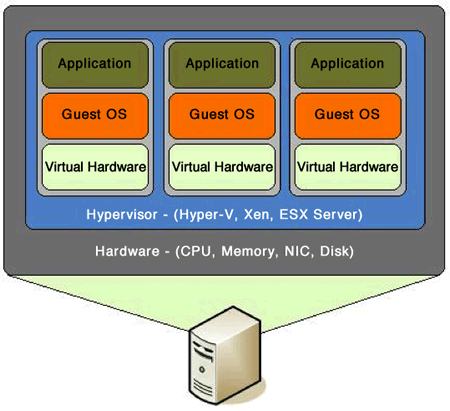
\includegraphics[scale = 0.5]{virtual_machine.png}
	\caption{\textit{virtual machine}}
	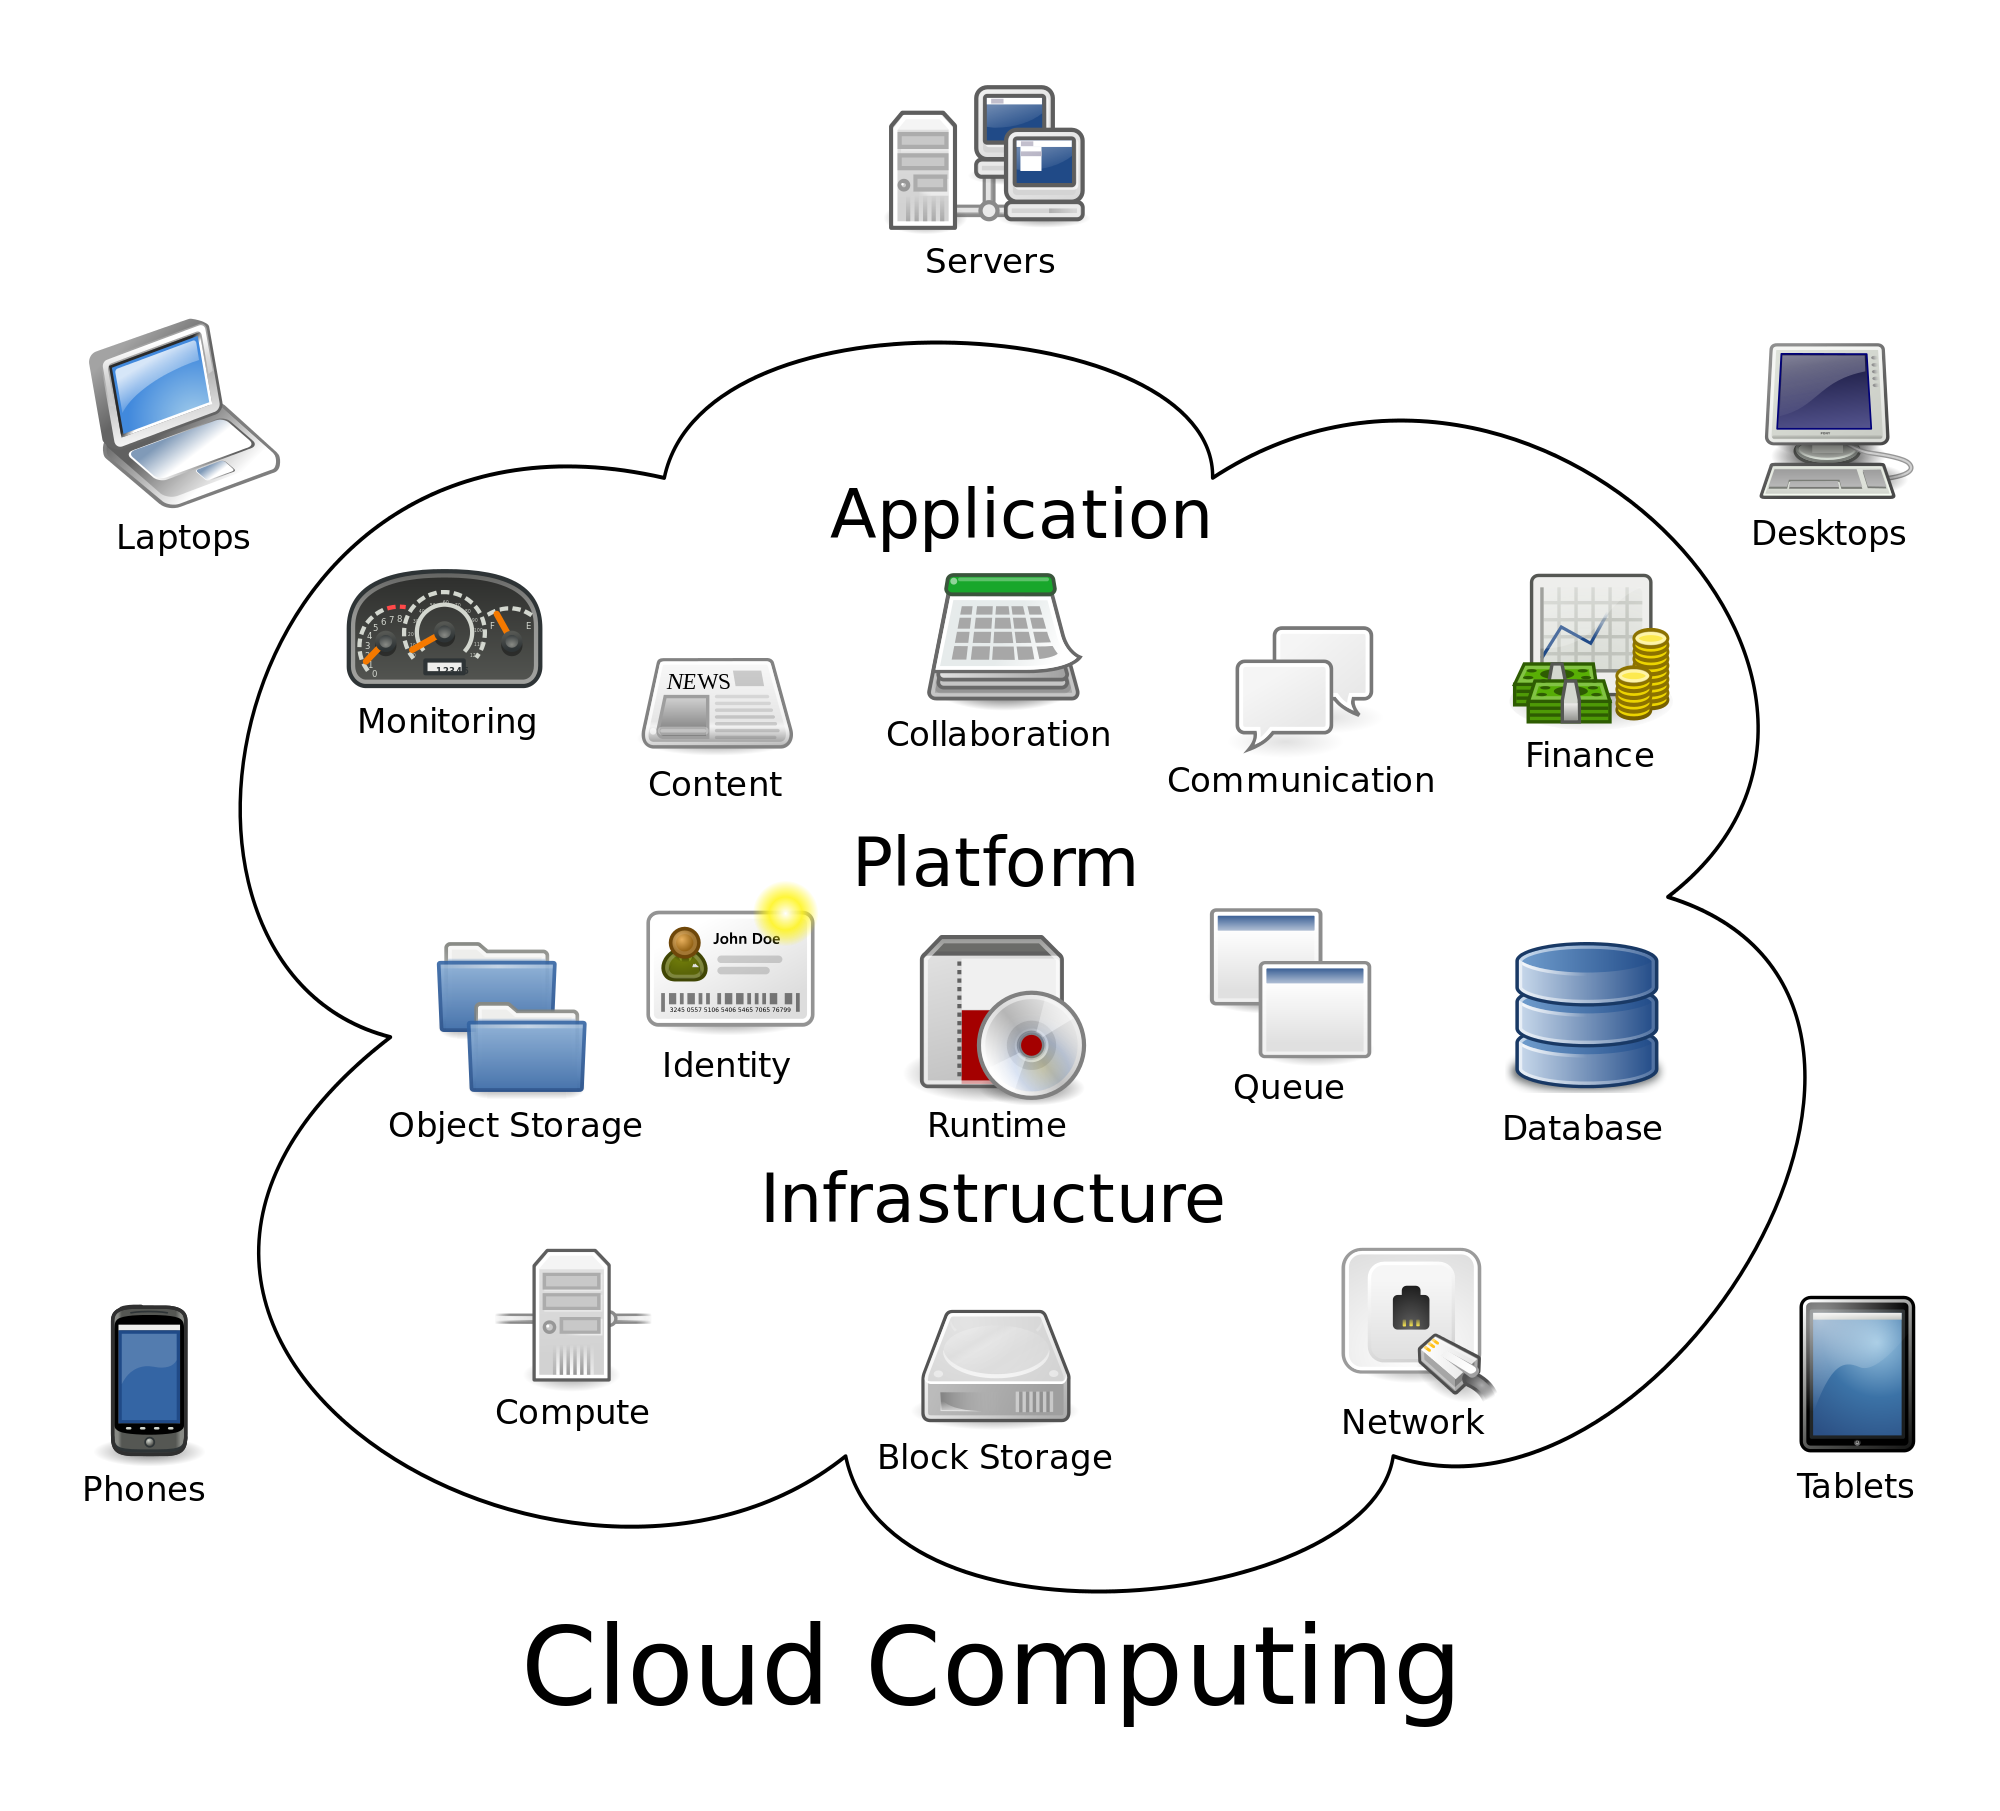
\includegraphics[scale = 0.1]{cloud_computing.png}
	\caption{\textit{cloud computing}}
\end{figure}
Salah satu bidang penelitian terkini yang menggunakan teknologi informasi dengan komputasi
tinggi adalah \textit{drug discovery}. Teknik terkait yang digunakan adalah 
\textit{virtual screening}, baik itu secara \textit{ligand-based} atau \textit{structured-based}
. Pemanfaatan teknologi \textit{cloud computing} diharapkan dapat memberikan kemudahan
bagi para peneliti tanpa perlu mempelajari secara detail pengoperasian dan perawatan teknologi yang mereka gunakan secara mendalam dan mengurangi kendala biaya dalam pengadaan \textit{supercomputer}. Dengan adanya \textit{cloud computing} peneliti juga dapat saling berbagi
\textit{resource}.

%-----------------------------------------------------------------------------%
\section{Permasalahan}
%-----------------------------------------------------------------------------%
%-----------------------------------------------------------------------------%
\subsection{Definisi Permasalahan}
%-----------------------------------------------------------------------------%
Berdasarkan latar belakang yang telah dijelaskan, penulis berusaha untuk menganalisis
apakah pemanfaatan Docker sebagai salah satu aplikasi abstraksi komputer secara \textit{virtual} dapat diajukan sebagai solusi alternatif
yang dapat digunakan dalam penelitian, khususnya terkait \textit{drug discovery}. 
Pengadaan \textit{supercomputer} secara fisik tentunya akan memakan alokasi tempat maupun biaya dalam penelitian.
Selain itu, dengan adanya \textit{cloud computing}, peneliti tidak dituntut untuk memahami
teknologi terkait secara mendalam, cukup fokus dengan penelitian yang sedang dikerjakan. Peneliti juga dapat dengan mudah saling berbagi \textit{resource}, baik itu sumber komputasi maupun data mentah maupun yang telah diolah.  
Aplikasi yang digunakan dalam tugas akhir ini adalah Autodock dan Autodock Vina bertugas untuk \textit{virtual screening}.


%-----------------------------------------------------------------------------%
\subsection{Batasan Permasalahan}
%-----------------------------------------------------------------------------%
Pada penelitian ini, penulis tidak akan berfokus pada \textit{virtual screening} yang akan dilakukan.Penulis mencoba untuk menganalasis apakah kinerja Docker setara atau lebih baik dibandingkan dengan \textit{cluster} dan 
\textit{grid computing} dalam melakukan \textit{drug discovery}. 


%-----------------------------------------------------------------------------%
\section{Tujuan}
%-----------------------------------------------------------------------------%
Penelitian ini secara umum bertujuan untuk mengenalkan pemanfaatan abstraksi komputer secara \textit{virtual} dibantu dengan teknologi \textit{cloud computing}
sebagai alternatif pengadaan \textit{supercomputer} secara fisik terkait dengan penelitian dengan menggunakan komputasi yang tinggi, khususnya \textit{drug discovery}
dalam bidang farmakologi. Selain itu, Penelitian ini secara khusus untuk menganalisis kinerja Docker
dalam menjalankan Autodock maupun Autodock Vina.


%-----------------------------------------------------------------------------%
\section{Posisi Penelitian}
%-----------------------------------------------------------------------------%
Penelitian ini merupakan lanjutan dari topik yang sedang dilakukan oleh Bapak Muhammad Hafizhuddin Hilman, S.Kom., M.Kom. 

%-----------------------------------------------------------------------------%
\section{Sistematika Penulisan}
%-----------------------------------------------------------------------------%
Penulisan ini terbagi dalam 5 bab :
\begin{itemize}
	\item BAB 1 \babSatu \\
	Bagian ini berisikan latar belakang, permasalahan, tujuan dan ruang lingkup penelitian, serta sistematika penulisan tugas akhir penelitian. 
	\item BAB 2 \babDua \\
	Bagian ini berisikan penjelasan \textit{drug discovery} dengan cara \textit{virtual screening} memanfaatkan teknologi informasi secara umum. Selain itu, \textit{cloud computing} dan Docker akan dijelaskan secara detail.
	\item BAB 3 \babTiga \\
	Bagian ini berisikan detail tahap-tahap penelitian dan data yang digunakan.
	\item BAB 4 \babEmpat \\
	Bagian ini berisikan hasil dari penelitian yang telah dilaksanakan dan analisis dari hasil yang diperoleh.
	\item BAB 5 \kesimpulan \\
	Bagian ini berisikan kesimpulan penulis terkait dengan penelitian dan saran penulis dalam penelitian ke depannya.
\end{itemize}



%-----------------------------------------------------------------------------%
\chapter{\babDua}
%-----------------------------------------------------------------------------%
Bab ini akan menjelaskan sekilas tentang \textit{computational drug discovery}, apa itu \textit{cloud computing} , dan Docker sebagai platform virtualisasi komputer. 
%-----------------------------------------------------------------------------%
\section{\textit{Computational Drug discovery}}
%-----------------------------------------------------------------------------%
\hspace{0.5cm}\textit{Drug discovery} adalah suatu proses menemukan kandidat obat yang berpotensial. Proses ini melibatkan berbagai displin ilmu seperti biologi, kimia, maupun farmakologi. Dalam \textit{drug discovery} dahulu kala, terkadang obat tersebut ditemukan secara tidak sengaja(\textit{serendipity}) atau berdasarkan penyembuhan tradisional. Seiring dengan berkembangnya pengetahuan dan teknologi, khususnya dalam bidang kimia, ekstraksi senyawa kimia dari makhluk hidup merupakan hal yang wajar. Ekstrak tersebut akan disimpan dan akan disimpan sebagai dalam suatu \textit{library} yang nantinya dapat digunakan kembali. Ekstrak tersebut dapat di-\textit{screening}, apakah terdapat senyawa yang berpotensi sebagai penyembuh dari suatu \textit{sympton} penyakit. Hal ini merupakan dasar farmakologi (\textit{classical pharmacology}).

Waktu yang dibutuhkan dalam proses \textit{drug discovery} cukup lama. Tidak hanya itu, proses ini juga sangat beresiko dan membutuhkan dana yang besar [1].Walaupun demikian, investasi dana dalam \textit{drug discovery} juga berkembang pesat. Namun, investasi tersebut tidak dibarengi dengan hasil yang proporsional dengan investasi tersebut. Hal ini disebabkan oleh rendahnya efektivitas dan tingginya kemungkinan kegagalan dalam \textit{drug discovery}. Beberapa pendekatan telah dilakukan dalam meningkatkan efektivitas, salah satu cara tersebut adalah CADD (\textit{Computer Aided Drug Design}).Dengan begitu, penekanan biaya dan siklus waktu penemuan obat juga semakin cepat. Dalam CADD, komputer digunakan sebagai sarana komputasi dan penyimpanan data dalam \textit{drug discovery}. Tidak ketinggalan, CADD menggunakan aplikasi dalam mendesain ikatan kimiawi, memodelkan struktur kimia yang mengandung kandidat calon obat yang berpotensial dan pembuatan \textit{library} yang dapat digunakan untuk pembelajaran selanjutnya.
\begin{figure}
	\centering
	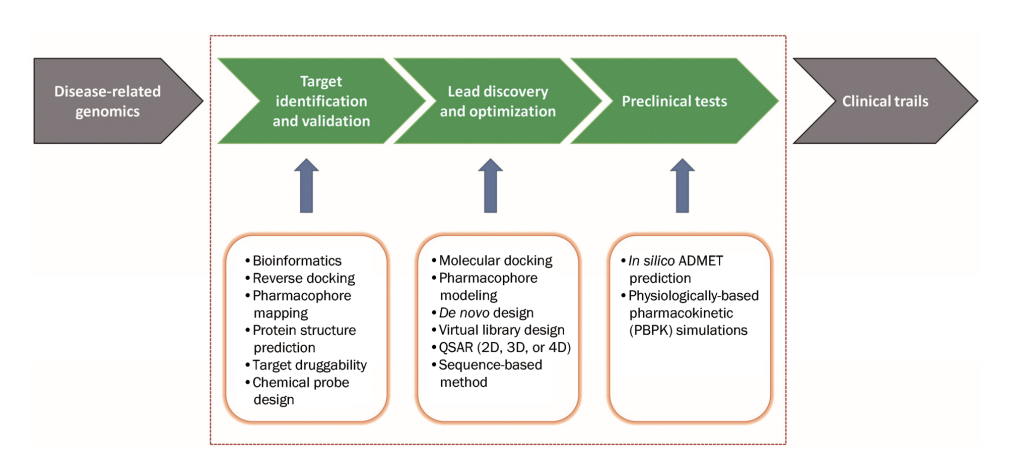
\includegraphics [scale=0.4]{siklus_dd.png}
	\caption{Pemanfaatan komputer sebagai sarana komputasi dalam \textit{drug discovery}}
\end{figure}
Dalam \textit{computational drug discovery} (penemuan obat dengan memanfaatkan komputer), pendekatan yang dapat dilakukan dibagi menjadi \textit{structure-based drug design}(SBDD), \textit{ligand-based drug design}(LBDD) dan pendekatan berdasarkan sekuens.  terdiri dari proses \textit{docking} kandidat \textit{ligand} ke target protein kemudian dilakukan penilaian dengan menggunakan \textit{scoring function} untuk dapat menghitung kemungkinan \textit{ligand}tersebut terikat pada target protein dengan daya tarik yang tinggi. 
\begin{figure}
	\centering
	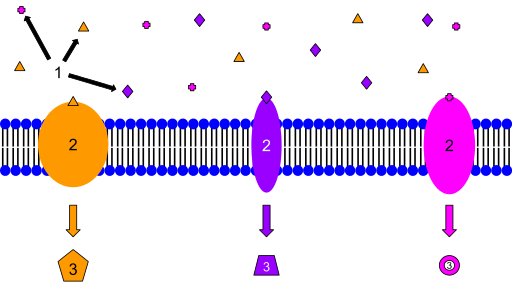
\includegraphics [scale=0.5]{receptor.png}
	\caption{Ilustrasi \textit{ligand}(nomor 1)yang akan terikat dengan \textit{receptor}(nomor 2)}
\end{figure}   
Dalam LBDD, diberikan sekumpulan \textit{ligand} dan \textit{receptor}, dimana model \textit{receptor}dapat dibuat dengan mengumpulkan informasi dari \textit{ligand}. Model ini dikenal dengan \textit{pharmacophore}. Kemudian, kandidat \textit{ligand} akan dibandingkan dengan \textit{pharmacophore}, apakah kompatibel dengan \textit{pharmacophore} dan dapat terikat.
\begin{figure}
	\centering
	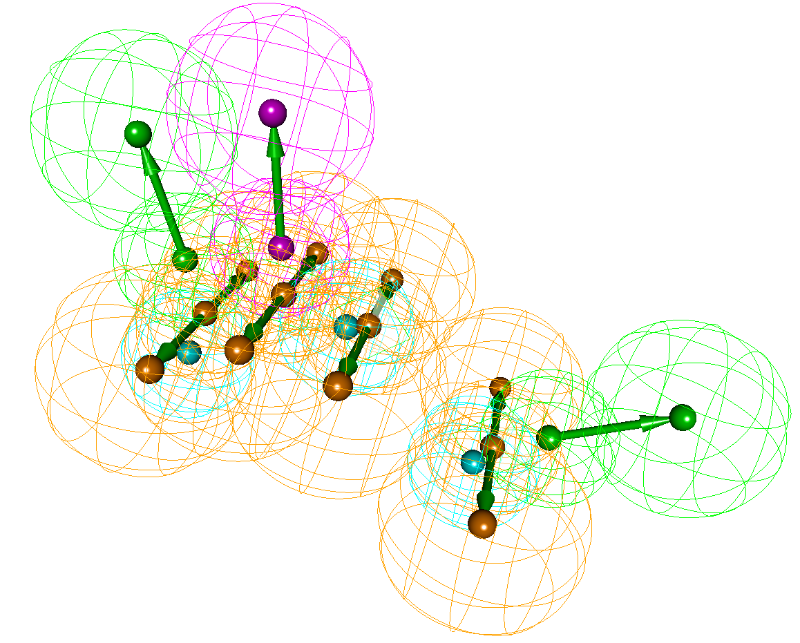
\includegraphics [scale=0.3]{pharmacophore.png}
	\caption{Contoh dari \textit{pharmacophore}}
\end{figure}  

\section{\textit{Molecular Docking}}
%-----------------------------------------------------------------------------%

\textit{Virtual screening} berdasarkan \textit{molecular docking} merupakan metode yang sering digunakan dalam SBDD. Penulis juga akan menggunakan metode tersebut yang terdapat dalam Program Autodock dan Autodock Vina. Pemodelan struktur kimia menggunakan \textit{molecular modeling} untuk mempelajari fenomena dari struktur kimia tersebut. Kemudahan dalam \textit{molecular modeling} sekarang ini dibantu dengan aplikasi komputer yang tersedia, namun masih terdapat kesulitan yaitu bagaiman cara mendapatkan model struktur ikatan kimia yang benar dan interpretasi model yang tepat.Secara umum, \textit{molecular modeling} dapat dikatakan sebagai pemanfaatan komputer dalam mengkonstruksi molekul dan melakukan berbagai macam perhitungan untuk mempelajari karakteristik dan sifat struktur ikatan kimia. Istilah \textit{molecular modeling} terkadang disamakan dengan istilah \textit{computational chemistry}.

Proses \textit{drug discovery} yang semula berupa \textit{trial and error} berubah menjadi proses yang dibantu dengan perhitungan komputer. Perhitungan tersebut digunakan dalam menentukan struktur ikatan kimia baru berdasarkan struktur protein yang sudah diketahui. Pendekatan ini terbagi menjadi dua : \textit{de novo design} dan \textit{docking}. \textit{Docking} merupakan suatu proses untuk menebak struktur \textit{complex} dari struktur \textit{ligand} dan protein. Dalam \textit{molecular modeling}, \textit{docking} dapat dipandang sebagai suatu metode untuk memprediksi orientasi suatu molekul ketika diikat dengan molekul lainnya untuk membentuk \textit{complex} yang stabil.  
\begin{figure}
	\centering
	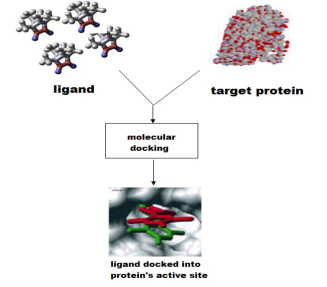
\includegraphics{docking.png}
	\caption{\textit{Proses molecular docking }}
\end{figure}

\textit{Molecular docking} adalah suatu proses komputasi dalam pencarian \textit{ligand} yang paling cocok baik secara geometri maupun energi ketika diikat dengan suatu \textit{receptor}(protein) yang telah diketahui.Aspek utama dalam \textit{molecular docking} adalah perhitungan energi interaksi dan konformasi dengan menggunakan metode dari kuantum mekanik hingga fungsi empiris energi. Permasalahan \textit{molecular docking} sekilas dapat dilihat sebagai suatu permasalahan \textit{lock and key}, dimana \textit{receptor} protein dapat dipandang sebagai \textit{lock} dan \textit{ligand} sebagai \textit{key}. Namun dalam praktiknya, \textit{molecular docking} akan mencari \textit{ligand} yang dapat menyesuaikan dengan \textit{receptor}.karena adaptasi tersebut, \textit{molecular docking} dapat dipandang sebagai permasalahan "\textit{best-fit}" \textit{ligand}. Diperlukan \textit{scoring function} untuk dapat membatasi \textit{best-fit} dari proses \textit{molecular docking}. Fungsi tersebut biasanya berdasarkan \textit{force field} yang digunakan dalam mensimulasikan protein. Beberapa \textit{scoring function} juga menambahkan aspek perhitungan lainnya seperti entropi.
\begin{figure}
	\centering
	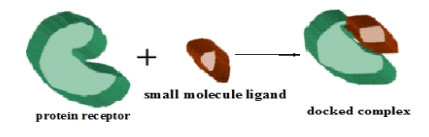
\includegraphics{molecular_docking.png}
	\caption{\textit{best-fit docking}}
\end{figure}
Dalam percobaan ini penulis memanfaatkan aplikasi \textit{molecular docking} Autodock dan Autodock Vina.

\section{\textit{Autodock dan Autodock Vina}}
%-----------------------------------------------------------------------------%
\hspace{0.5cm}Aplikasi ini merupakan aplikasi yang dikembangkan oleh \textit{The Scripps Research Institute}, lembaga riset nonprofit yang terletak di California, Amerika Serikat.
%-----------------------------------------------------------------------------%
\chapter{\babTiga}
%-----------------------------------------------------------------------------%
\todo{tambahkan kata-kata pengantar bab 1 disini}


%-----------------------------------------------------------------------------%
\section{Satu Persamaan}
%-----------------------------------------------------------------------------%

\noindent \begin{align}\label{eq:garis}
	\cfrac{y - y_{1}}{y_{2} - y_{1}} = 
	\cfrac{x - x_{1}}{x_{2} - x_{1}}
\end{align}

\equ~\ref{eq:garis} diatas adalah persamaan garis. 
\equ~\ref{eq:garis} dan \ref{eq:bola} sama-sama dibuat dengan perintah \bslash
align. 
Perintah ini juga dapat digunakan untuk menulis lebih dari satu persamaan. 

\noindent \begin{align}\label{eq:bola}
	\underbrace{|\overline{ab}|}_{\text{pada bola $|\overline{ab}| = r$}} 
		= \sqrt[2]{(x_{b} - x_{a})^{2} + (y_{b} - y_{a})^{2} + 
				\vert\vert(z_{b} - z_{a})^{2}}
\end{align}

%-----------------------------------------------------------------------------%
\section{Lebih dari Satu Persamaan}
\label{sec:multiEqu}
%-----------------------------------------------------------------------------%
\noindent \begin{align}\label{eq:matriks}	
	|\overline{a} * \overline{b}| &= |\overline{a}| |\overline{b}| \sin\theta 
		\\[0.2cm]
	\overline{a} * \overline{b} &=  
		\begin{array}{| c c c |}
			\hat{i} & x_{1} & x_{2} \\
			\hat{j} & y_{1} & y_{2} \\
			\hat{k} & z_{1} & z_{2} \\
		\end{array} \nonumber \\[0.2cm]
	&= \hat{i} \,
		\begin{array}{ | c c | }
			y_{1} & y_{2} \\
			z_{1} & z_{2} \\
		\end{array} 
	   + \hat{j} \,
		\begin{array}{ | c c | }
			z_{1} & z_{2} \\
			x_{1} & x_{2} \\
		\end{array} 
	   + \hat{k} \,	
		\begin{array}{ | c c | }
			x_{1} & x_{2} \\
			y_{1} & y_{2} \\
		\end{array}
		\nonumber
\end{align}

Pada \equ~\ref{eq:matriks} dapat dilihat beberapa baris menjadi satu bagian 
dari \equ~\ref{eq:matriks}. 
Sedangkan dibawah ini dapat dilihat bahwa dengan cara yang sama, \equ~
\ref{eq:gabungan1}, \ref{eq:gabungan2}, dan \ref{eq:gabungan3} memiliki nomor 
persamaannya masing-masing. 

\noindent \begin{align}\label{eq:gabungan1}	
	\int_{a}^{b} f(x)\, dx + \int_{b}^{c} f(x) \, dx = \int_{a}^{c} f(x) \, dx
		\\\label{eq:gabungan2}
	\lim_{x \to \infty} \frac{f(x)}{g(x)} = 0 \hspace{1cm} 
		\text{jika pangkat $f(x)$ $<$ pangkat $g(x)$} \\\label{eq:gabungan3}
	a^{m^{a \, ^{n}\log b }} = b^{\frac{m}{n}}
\end{align}


%-----------------------------------------------------------------------------%
\chapter{\babEmpat}
%-----------------------------------------------------------------------------%
Bab ini akan membahas hasil penelitian yang telah dilakukan dan analisis terhadap
hasil penelitian tersebut. 

%-----------------------------------------------------------------------------%
\section{Hasil Penelitian}
%-----------------------------------------------------------------------------%
\hspace{0.5cm}Berdasarkan kerangka penelitian yang telah dijelaskan pada bab sebelumnya, terdapat 10 skenario percobaan dimana masing - masing 5 skenario pada aplikasi Autodock dan 5 skenario pada aplikasi Autodock Vina. Secara garis besar, skenario tersebut adalah menjalankan aplikasi yang telah terpasang pada \textit{container} Docker yang telah dibuat. Untuk setiap skenario jumlah data pada masing - masing \textit{container} akan dibagi berdasarkan total data (1406 data \textit{receptor}) dibagi dengan jumlah \textit{container} yang terbentuk. Setelah data terbagi, masing - masing \textit{container} akan menjalankan aplikasi (Autodock ataupun Autodock Vina) dan waktu akan dicatat dari awal eksekusi data pertama hingga waktu akhir ketika aplikasi selesai mengeksekusi data terakhir.

Berikut merupakan data yang diperoleh dari 5 skenario aplikasi Autodock Vina

\begin{table}[h]
	\centering
	\begin{tabular}{|c|l|l|l|}
		\hline
		\multirow{2}{*}{Jumlah \textit{container}} & \multicolumn{3}{c|}{Waktu eksekusi (menit)} \\ \cline{2-4} 
		& \multicolumn{1}{c|}{tercepat} & \multicolumn{1}{c|}{terlama} & \multicolumn{1}{c|}{Rata-rata} \\ \hline
		50 & 625 & 1359 & 968 \\ \hline
		100 & 407 & 1434 & 891 \\ \hline
		150 & 247 & 2615 & 745 \\ \hline
		200 & 129 & 1496 & 705 \\ \hline
		250 & 193 & 1431 & 720 \\ \hline
	\end{tabular}
		\caption{Hasil skenario eksperimen pada aplikasi Autodock Vina}
		\label{my-label}
\end{table}

Untuk masing - masing data waktu eksekusi tersebut dapat disajikan menjadi tabel grafik. Tabel yang disajikan berupa waktu eksekusi tercepat, terlama dan rata - rata eksekusi setiap \textit{container} untuk setiap skenario.

\begin{figure}
	\centering
	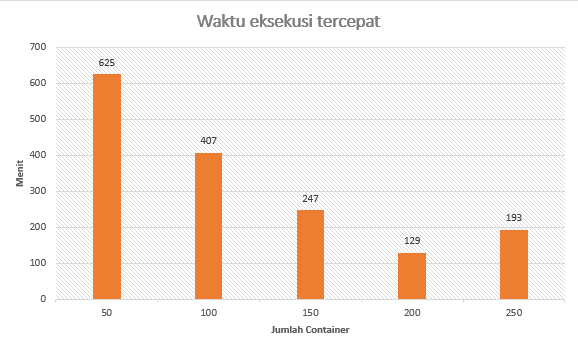
\includegraphics{tercepat_vina.PNG}
	\caption{Waktu eksekusi tercepat untuk masing - masing skenario Autodock Vina}
\end{figure}
 
\begin{figure}
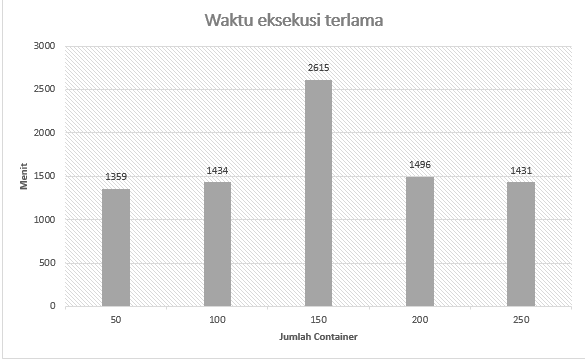
\includegraphics{terlama_vina.PNG}
\caption{Waktu eksekusi terlama untuk masing - masing skenario Autodock Vina}
\end{figure}

\begin{figure}
	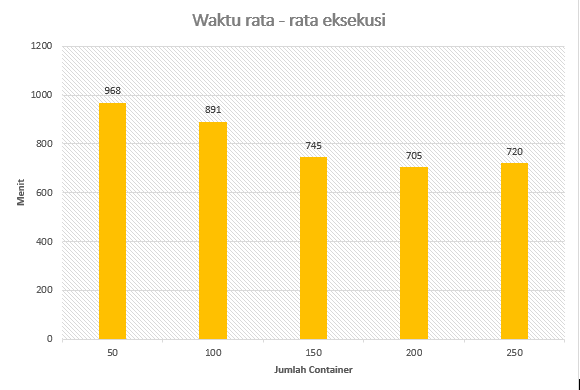
\includegraphics{ratarata_vina.PNG}
	\caption{Grafik dari rata - rata waktu eksekusi masing - masing skenario Autodock Vina}
\end{figure}

Berikut merupakan data yang diperoleh dari 5 skenario aplikasi Autodock 
\begin{table}
	\centering
	\begin{tabular}{|c|l|l|l|}
		\hline
		\multirow{2}{*}{Jumlah \textit{container}} & \multicolumn{3}{c|}{Waktu eksekusi (menit)} \\ \cline{2-4} 
		& \multicolumn{1}{c|}{tercepat} & \multicolumn{1}{c|}{terlama} & \multicolumn{1}{c|}{Rata-rata} \\ \hline
		50 & 1044 & 1344 & 1255 \\ \hline
		100 & 835 & 1386 & 1259 \\ \hline
		150 & 710 & 1405 & 1216 \\ \hline
		200 & 482 & 1276 & 1007 \\ \hline
		250 & 358 & 1071 & 811 \\ \hline
	\end{tabular}
	\caption{Hasil skenario pada eksperimen Autodock}
	\label{my-label}
\end{table}

Untuk masing - masing data waktu eksekusi tersebut dapat disajikan menjadi tabel grafik :

\begin{figure}
	\centering
	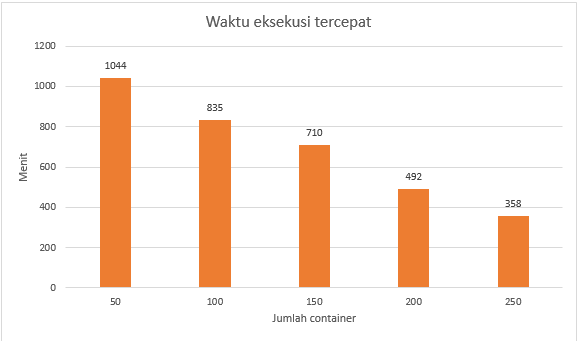
\includegraphics{tercepat_dock.PNG}
	\caption{Waktu eksekusi tercepat untuk masing - masing skenario Autodock}
\end{figure}

\begin{figure}
	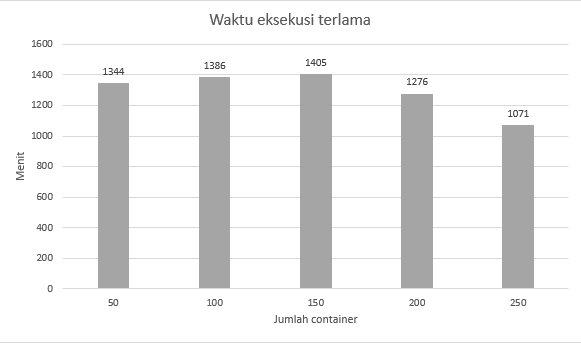
\includegraphics{terlama_dock.PNG}
	\caption{Waktu eksekusi terlama untuk masing - masing skenario Autodock}
\end{figure}

\begin{figure}
	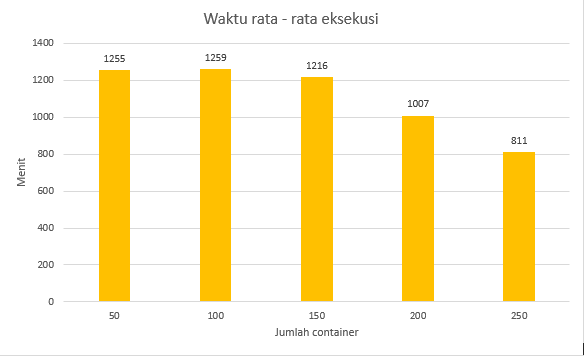
\includegraphics{ratarata_dock.PNG}
	\caption{Grafik rata - rata waktu eksekusi masing - masing skenario Autodock}
\end{figure}

%-----------------------------------------------------------------------------%
\section{Analisis}
%-----------------------------------------------------------------------------%
\hspace{0.5cm}Pada situs resmi Autodock telah ditampilkan perbandingan performa antara Autodock dan Autodock Vina \cite{comparison_dockvina} seperti berikut :
 
\begin{figure}
	\centering
	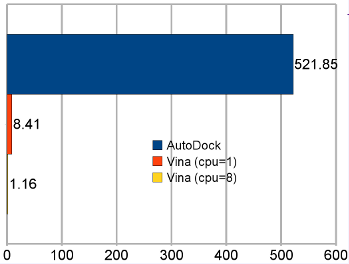
\includegraphics{comparison_dockvina.PNG}
	\caption{Perbandingan waktu \textit{running} pada situs resmi Autodock \cite{autodockvina}}
\end{figure}

Eksekusi pada Autodock Vina jauh lebih cepat dibandingkan dengan Autodock, hal ini dikarenakan pada aplikasi Autodock Vina memanfaatkan \textit{multithreading} sehingga dapat mengoptimalkan kinerja dari banyak CPU \cite{autodockvina}. Gambar 4.7 diatas memberikan gambaran awal bahwa dalam skenario penelitian yang dilakukan, Autodock Vina akan memberikan waktu eksekusi yang lebih cepat dibandingkan dengan Autodock. Untuk setiap rata - rata waktu eksekusi pada skenario Autodock Vina dibandingkan dengan rata - rata waktu eksekusi pada skenario Autodock memberikan hasil yang sama dengan grafik yang diberikan pada situs resmi Autodock.

Pada tabel waktu rata - rata eksekusi untuk aplikasi Autodock dan Autodock Vina dapat dilihat bahwa grafik dari setiap skenario memberikan \textit{trend} menurun. Dengan begitu dapat dilihat bahwa jumlah \textit{container} dan jumlah data menjadi faktor yang mempengaruhi waktu proses tersebut. Dapat disimpulkan bahwa, semakin banyak \textit{container} yang dibentuk maka semakin sedikit data yang digunakan pada aplikasi Autodock maupun Autodock Vina pada masing - masing \textit{container}. Semakin banyak \textit{container} juga memperbanyak eksekusi aplikasi yang dilakukan secara paralel. Pada gambar  grafik 4.3 dan 4.6 diatas terlihat \textit{trend} semakin banyak \textit{container} maka waktu eksekusi akan semakin sedikit. Namun dapat dilihat juga pada gambar tabel 4.3, \textit{container} 200 menghasilkan waktu eksekusi yang lebih kecil dibandingkan dengan \textit{container} 250. Penulis memperkirakan bahwa kompleksitas molekul juga mengambil andil dalam lamanya waktu yang dibutuhkan oleh aplikasi Autodock maupun Autodock Vina. Untuk dapat memastikan bahwa jumlah \textit{container} mempengaruhi, penulis mencoba untuk menghitung waktu eksekusi aplikasi Autodock dan Autodock Vina dalam memproses 1406 data receptor.

\begin{table}
	\centering
	\begin{tabular}{|c|c|c|}
		\hline
		\multicolumn{3}{|c|}{Waktu eksekusi (menit)} \\ \hline
		Jumlah Container & Autodock & Autodock Vina \\ \hline
		1 & 4797 & 1459 \\ \hline
	\end{tabular}
	\caption{Waktu eksekusi Autodock dan Autodock Vina saat 1 \textit{container}}
	\label{my-label}
\end{table}

Dapat dilihat pada tabel 4.3 bahwa waktu yang dibutuhkan dalam menjalankan skenario percobaan dengan hanya menggunakan 1 buah \textit{container} memakan waktu yang lebih lama dibandingkan dengan banyak \textit{container} pada skenario penelitian.

Dari skenario yang telah dilakukan, penulis juga mengamati kinerja CPU dan memori yang digunakan oleh Docker. Berdasarkan penjelasan Marek Goldmann \cite{Marek Goldmann} , setiap \textit{container} yang dibentuk akan membagi sama rata \textit{resource} CPU. Pembagian tersebut hanyalah \textit{relative weight}, dimana setiap \textit{container} dapat menggunakan \textit{shared} CPU, bukan kecepatan kasar CPU yang digunakan oleh \textit{container}. Container yang terbentuk awalnya akan memiliki 1024 \textit{shared} CPU dari CPU fisik, dan akan terbagi sama rata selama \textit{container} baru akan terbentuk. Hasil dari penelitian ini baik menjalankan aplikasi Autodock maupun Autodock Vina dapat dilihat sebagai berikut :
\begin{table}
	\centering
	\begin{tabular}{|c|c|c|}
		\hline
		\multicolumn{3}{|c|}{\textit{Relative weight} CPU (\%)} \\ \hline
		Jumlah \textit{container} & Autodock Vina & Autodock \\ \hline
		50 & 15,9 - 16,9 & 15,6 -19,6 \\ \hline
		100 & 7,9 - 12,3 & 8 - 8,6 \\ \hline
		150 & 5 - 5,6 & 6-7,6 \\ \hline
		200 & 3,3 - 3,9 & 4,6 - 5 \\ \hline
		250 & 0,7 - 3 & 3,6 - 4 \\ \hline
	\end{tabular}
	\caption{Persentasi \textit{relative weight} pemanfaatan CPU}
	\label{my-label}
\end{table}

Walaupun dari tabel diatas tidak seperti perhitungan yang dikatakan oleh Marek Goldmann, angka - angka tersebut tetap mendekati pembagian secara merata. Penelitian yang dilakukan menggunakan \textit{desktop} CPU dengan  prosesor Intel i-7 , dimana prosesor secara fisik memiliki 4 core namun dengan adanya \textit{Hyper Threading}, terdapat logical core untuk masing - masing core sehingga terbaca menjadi 8 core (800 \%). Dalam kenyataannya, nilai \textit{relative weight} dapat berubah mengikuti besarnya \textit{task} yang dikerjakan oleh \textit{container} tersebut dan nilai \textit{relative weight} \textit{container} lain. Nilai \textit{relative wieght container} dalam keadaan \textit{idle} dapat terbagi sama rata untuk \textit{container} lain yang masih mengerjakan \textit{task} (menyesuaikan dengan \textit{task} dalam \textit{container}). Dalam hal pembagian memori, setiap \textit{container} dapat menggunakan memori pada \textit{host} hingga kapasitas maksimum memori pada \textit{host}. Pada eksperimen yang dijalankan, terlihat bahwa untuk aplikasi Autodock Vina maupun Autodock yang dijalankan hanya menggunakan 0,1 \% - 0,9 \% dari memori pada komputer \textit{host}

Dalam penelitian ini penulis juga membandingkan performa yang diberikan oleh Docker dengan penelitian yang telah dilakukan oleh Muhammad H. Hilman \cite{cloud_pak hilman}. Beliau menggunakan aplikasi Autodock Vina dalam \textit{virtual screening}. Perbandingan dilakukan dengan mencari waktu untuk memproses 1 buah molekul. Waktu ini didapat dengan membagi waktu yang dihasilkan dari awal eksekusi aplikasi Autodock maupun Autodock Vina pada \textit{container} hingga aplikasi selesai bekerja dengan jumlah data yang digunakan dalam eksperimen penelitian, yaitu 1406 buah data. Berikut merupakan gambar tabel waktu yang dibutuhkan dalam memproses 1 molekul yang dapat dikerjakan dalam \textit{virtual cluster} dalam Amazon EC2 :
\begin{table}
	\centering
	\begin{tabular}{|c|c|c|c|}
		\hline
		Parameter & SCluster & LCluster & XLCluster \\ \hline
		Memory & 1,7 GB & 7,5GB & 15 GB \\ \hline
		Compute Unit / Processors & 1,2 GHz X 1 & 1,2 GHz X 4 & 1,2 GHz X 8 \\ \hline
		Platform & 32-bit & 64-bit & 64-bit \\ \hline
		Harga/jam & \$0,085 & \$0,34 & \$0,68 \\ \hline
	\end{tabular}
\caption{Spesifikasi harga dan \textit{resource cloud computing} yang disediakan oleh Amazon EC2 \cite{cloud_pak hilman}}
	\label{my-label}
\end{table}
Berdasarkan penelitian yang dilakukan sebelumnya, masing - masing \textit{cluster} terdiri dari 4 node. \textit{Hardware} komputasi tidak sama untuk masing - masing \textit{cluster}, Amazon memberikan gambaran besarnya \textit{clock speed} dan berapa jumlah \textit{processor}.  
\begin{table}
	\centering
	\begin{tabular}{|l|l|l|l|}
		\hline
		Parameter & SCluster & LCluster & XLCluster \\ \hline
		Total ExecTime(s) & 375.624 & 108.179 & 48.421 \\ \hline
	\end{tabular}
	\caption{Hasil pengukuran \textit{virtual screening} \cite{cloud_pak hilman}}
	\label{my-label}
\end{table}
Tabel diatas merupakan hasil waktu yang diperoleh dalam menjalankan Autodock Vina pada jasa \textit{cloud computing} Amazon EC2. Waktu yang dihasilkan dihitung dalam ribuan detik. Untuk menghitung waktu eksekusi 1 molekul dapat dibagi dengan banyaknya molekul yang digunakan, 1406 molekul. Dengan begitu didapatkan tabel berikut :
\begin{table}
	\centering
	\begin{tabular}{|c|c|c|c|}
		\hline
		\multicolumn{4}{|c|}{Pemrosesan 1 Molekul dalam detik (s)} \\ \hline
		Parameter & SCluster & LCluster & XLCluster \\ \hline
		AvgExecTime(s) & 267 & 77 & 34 \\ \hline
	\end{tabular}
	\caption{Waktu yang dibutuhkan dalam memproses 1 buah Molekul berdasarkan tabel 4.6 diatas}
	\label{my-label}
\end{table}
Hasil yang diperoleh dari eksperimen penelitian ini :
\begin{table}
	\centering
	\begin{tabular}{|c|c|}
		\hline
		\multicolumn{2}{|c|}{Pemrosesan 1 Molekul dalam detik (s)} \\ \hline
		Jumlah \textit{container} & Autodock Vina \\ \hline
		1 & 62,26 \\ \hline  
		50 & 41,30 \\ \hline
		100 & 38,02 \\ \hline
		150 & 32,19 \\ \hline
		200 & 30,08 \\ \hline
		250 & 31,02 \\ \hline
	\end{tabular}
	\caption{Waktu yang dibutuhkan dalam memproses 1 buah Molekul}
	\label{my-label}
\end{table}

Dapat dilihat bahwa hasil yang diberikan oleh Docker pada sebuah \textit{desktop} PC tidak jauh berbeda dengan yang diberikan oleh Amazon EC2 . Dari tabel tersebut dapat dilihat dalam eksekusi pada Docker dengan \textit{container} terkecil dapat memberikan hasil yang lebih cepat dibandingkan dengan LCluster. Waktu tercepat masih dipegang oleh XLCluster, namun hasil yang diberikan oleh Docker dapat mendekati \textit{virtual cluster} yang digunakan oleh Amazon EC2.

Untuk memastikan bahwa penggunaan \textit{platform} Docker dapat mengoptimisasi kinerja CPU, penulis melakukan skenario tambahan dengan melakukan \textit{virtual screening} di atas \textit{desktop} PC yang digunakan pada percobaan.
\begin{table}
	\centering
	\label{my-label}
	\begin{tabular}{|c|c|c|}
		\hline
		\multicolumn{3}{|c|}{Waktu eksekusi pada komputer \textit{native}} \\ \hline
		Parameter & Autodock & Autodock Vina \\ \hline
		Waktu total (menit) & 4942,8 & 1460 \\ \hline
		Waktu per 1 molekul (detik) & 211,33 & 62,3 \\ \hline
	\end{tabular}
		\caption{Hasil \textit{virtual screening} yang berjalan pada komputer \textit{native}}
\end{table}

Dapat dilihat bahwa hasil yang diberikan mendekati hasil skenario ketika menjalankan \textit{virtual screening} pada 1 buah \textit{container} Docker. Semakin banyak \textit{container} yang digunakan maka persebaran data akan semakin sedikit. Menjalankan program secara paralel dengan data sedikit akan lebih cepat dibandingkan dengan menjalankan sebuah program dengan data yang banyak.Selain itu, dapat ditarik kesimpulan bahwa semakin banyak jumlah \textit{container}, \textit{overhead} yang akan terjadi semakin tinggi. Oleh karena itu, kemungkinan \textit{processor} dalam keadaan \textit{idle} akan semakin sedikit dibandingkan dengan menjalankan \textit{virtual screening} di atas komputer \textit{native} maupun dengan 1 buah \textit{container}

Dari segi pengeluaran biaya, pemanfaatan teknologi \textit{cloud computing} akan lebih murah dibandingkan dengan pengadaan komputer secara fisik. Hal ini disebabkan pihak penyedia jasa \textit{cloud computing} dalam hal ini Amazon EC2, memberikan daftar harga sesuai dengan \textit{resource} yang digunakan dibandingkan dengan membayar secara keseluruhan perangkat keras yang disediakan untuk pengguna. Penulis membandingkan kembali dari biaya \textit{cluster} yang dilakukan oleh Bapak Muhammad H. Hilman pada penelitian beliau \cite{cloud_pak hilman}
\begin{table}
	\centering
	\begin{tabular}{|l|l|l|l|}
		\hline
		Parameter & SCluster & LCluster & XLCluster \\ \hline
		Harga per jam (\$) & 0,085 & 0,0292 & 0.0252 \\ \hline
		Total Cost(\$) & 35,36 & 40,8 & 35,36 \\ \hline
		Average Cost(\$) & 0,0252 & 0,0292 & 0,0252 \\ \hline
	\end{tabular}
	\caption{Biaya yang dikeluarkan oleh Bapak Muhammad H. Hilman dalam penelitiannya \cite{cloud_pak hilman}}
	\label{my-label}
\end{table}

Pada tabel tersebut, average cost merupakan biaya yang dibutuhkan dalam memproses 1 buah molekul (Total Cost dibagi dengan 1406 molekul). Jika dilakukan kurs mata uang akan didapatkan Rp. 224,00 \textemdash \hspace{0.1 cm}Rp. 260,00 untuk 1 buah molekul. Dibandingkan dengan biaya penggunaan \textit{desktop} PC yang digunakan dalam penelitian ini. Karena tidak relevan menghitung biaya dengan sekali penggunaan \textit{virtual screening}, maka penulis menggunakan beberapa asumsi:
\begin{itemize}
	\item Umur ekonomis perangkat komputer berdasarkan Surat Edaran Direktur Jenderal Pajak Nomor SE-07/PJ.42/2002 tanggal 8 Mei 2002 adalah 4 tahun
	\item Penggunaan komputer untuk sebuah proyek \textit{virtual screening} 1 bulan (30 hari kerja) sehingga diperoleh 720 jam kerja
	\ Besarnya listrik yang digunakan oleh komputer 500 watt 
\end{itemize}
Dari asumsi tersebut akan didapatkan total biaya :
\begin{itemize}
	\item Biaya pengadaan komputer : Rp 14,250,000 (Berdasarkan spesifikasi komputer pada situs Bhinneka.com)
	\item Biaya maintenance sebesar 10 \% dari investasi : Rp 1,425,000
	\item Konsumsi listrik : 4 X 720 jam X 500 watt = 1440 kwh
	\item Biaya konsumsi listrik (tarif gol. pemerintahan): Rp. 23,800 per kwh x 2880 kwh = Rp 34,272,000
	\item Asumsi jika terjadi kerusakan, biaya teknisi 4 tahun x 1 bulan x Rp. 2,000,000 = Rp 8,000,000
\end{itemize}    
Maka total biaya yang dikeluarkan Rp 57,947,000. Untuk dapat mengetahui biaya per 1 molekul maka perlu dibagi dengan lamanya eksekusi \textit{virtual screening} 1 molekul. Dalam hal ini penulis menggunakan waktu autodock vina saat \textit{container} berjumlah 150. Didapatkan 1 buah molekul memakan waktu 32,19 detik.
\begin{itemize}
	\item Waktu kerja total = 4 tahun X 720 jam = 2880 jam
	\item Besarnya waktu kerja dalam satuan detik 2880 jam X 60 menit X 60 detik = 10.368.000 detik
	\item Banyaknya molekul yang diproses = 10.368.000 / 32,19 = 322.087 molekul 
\end{itemize}
Didapatkan Rp 57,947,000 / 322.087 molekul = Rp 179,911. Walaupun cukup murah, penggunaan komputer tersebut belum tentu penuh selama 4 tahun. Terdapat faktor lain yang dapat mempengaruhi seperti adanya proyek \textit{virtual screening}, putusnya sambungan listrik yang menyebabkan proyek \textit{virtual screening} perlu diulang kembali dari awal, dan lain sebagainya yang menghambat. Sedangkan dengan jasa \textit{cloud computing}, walaupun dari perhitungan lebih mahal dibandingkan dengan penggunaan komputer biasa, biaya yang dikeluarkan hanya saat menggunakan \textit{resource} komputasi saja dan kemungkinan terjadinya kegagalan pada perangkat keras tidak akan terjadi.





%---------------------------------------------------------------
\chapter{\kesimpulan}
%---------------------------------------------------------------
\todo{Tambahkan kesimpulan dan saran terkait dengan perkerjaan 
	yang dilakukan.}


%---------------------------------------------------------------
\section{Kesimpulan}
%---------------------------------------------------------------


%---------------------------------------------------------------
\section{Saran}
%---------------------------------------------------------------


%
% Daftar Pustaka
%
% Daftar Pustaka 
% 

% 
% Tambahkan pustaka yang digunakan setelah perintah berikut. 
% 
\begin{thebibliography}{4}

\bibitem{cluster_pak hilman}
{Muhammad H. Hilman.Juni 2010.\f{"Evaluasi Kinerja Autodock 4.2 dan Autodock Vina 1.1 dalam Proses Molecular Docking dan Virtual Screening di Lingkungan Cluster Hastinapura"}.Fakultas Ilmu Komputer,Universitas Indonesia.}

\bibitem{cloud_pak hilman}
{Muhammad H. Hilman.Januari 2012.\f{"Analisis Teknik Data Mining dan Kinerja
		Infrastruktur Komputasi Cloud Sebagai Bagian dari
		Sistem Perancangan Obat Terintegrasi"}.Fakultas Ilmu Komputer,Universitas Indonesia.}

\bibitem{Drugdiscovery}
{Pharma \f{Drug Discovery and Development : UNDERSTANDING THE R and D PROCESS}.February 2007.\url{http://www.phrma.org/sites/default/files/pdf/rd_brochure_022307.pdf}.}

\bibitem{Drugdiscovery2}
{Myers S, Baker A. \f{Drug discovery - an operating model for a new era}.Nat Biotechnol 2001; 19: 727–30}

\bibitem{doCADD}
{Matthew Segall.\f{Can we really do computer-aided drug design?}.J Comput Aided Mol Des (2012) 26:121–124}

\bibitem{reviewCADD}
{Si-sheng OU-YANG, Jun-yan LU, Xiang-qian KONG, Zhong-jie LIANG, Cheng LUO, Hualiang JIANG.\f{Review Computational drug discovery}.Acta Pharmacologica Sinica (2012) 33: 1131–1140}

\bibitem{diagram drug discovery}
{Gambar diagram drug discovery. Diambil dari artikel : Myers S, Baker A. \f{Drug discovery - an operating model for a new era}.Nat Biotechnol 2001; 19: 727–30 }

\bibitem{rankingSBDD}
{Rajamani R, Good AC.2007. \f{"Ranking poses in structure-based lead discovery and optimization: current trends in scoring function development"}.Current Opinion in Drug Discovery and Development 10 (3): 308–15.}

\bibitem{gambar MolecularDocking}
{Gambar ilustrasi molecular docking. Diambil dari artikel : Bachwani Mukesh, Kumar Rakesh.\f{Molecular Docking : A Review}.IJRAP (2011) 2 (6) 1746 - 1751.}

\bibitem{Drugdesign}
{\f{Drug design}. \url{http://strbio.biochem.nchu.edu.tw/classes/special_topics_biochem/course_ppts/rational_drug_design-2014.pdf}.diakses pada 3 Juni 2015 pukul 04:49}

\bibitem{MolecularDocking}
{Bachwani Mukesh, Kumar Rakesh.\f{Molecular Docking : A Review}.IJRAP (2011) 2 (6) 1746 - 1751.}

\bibitem{pharmacophore}
{Contoh model \textit{pharmacophore}.\url{http://en.wikipedia.org/wiki/Pharmacophore#/media/File:PharmacophoreModel_example.svg} diakses 3 Juni 2015 pukul 18:09}

\bibitem{De Novo}
{Schneider G, Fechner U.August 2005. \f{"Computer-based de novo design of drug-like molecules".} Nat Rev Drug Discov 4 (8): 649–63.}

\bibitem{Docking and Scoring}
{Kitchen DB, Decornez H, Furr JR, Bajorath J.2004.\f{"Docking and scoring in virtual screening for drug discovery: methods and applications"}.Nature reviews. Drug discovery 3 (11): 935–49.}

\bibitem{best-fit}
{Wei BQ, Weaver LH, Ferrari AM, Matthews BW, Shoichet BK.2004. \f{"Testing a flexible-receptor docking algorithm in a model binding site"}. J. Mol. Biol. 337 (5): 1161–82.}

\bibitem{autodock most cited}
{Morris.2007,May 04.\f{"AutoDock is the most cited docking software"} \url{http://autodock.scripps.edu/news/autodock-is-the-most-cited-docking-software} diakses 3 Juni 2015 pukul 06:59}

\bibitem{website resmi}
{Website resmi The Scripps Research Institute,
	\url{http://www.scripps.edu/about/index.html} diakses 6 Juni 2015 pukul 14.39}

\bibitem{autodock}
{Garrett M. Morris et al.2009.\f{"AutoDock4 and AutoDockTools4: Automated Docking with Selective Receptor Flexibility"}.J Comput Chem. 2009 December ; 30(16): 2785–2791. doi:10.1002/jcc.21256}

\bibitem{autodockvina}
{Oleg Trott and Arthur J. Olson.2010.\f{"AutoDock Vina: improving the speed and accuracy of docking	with a new scoring function, efficient optimization and multithreading"}.J Comput Chem. 2010 January 30; 31(2): 455–461. doi:10.1002/jcc.21334.}

\bibitem{Logo autodock}
{Logo Autodock. \url{http://www.kdm.wcss.wroc.pl/w/images/thumb/Autodock_logo.gif/200px-Autodock_logo.gif} diakses 3 Juni 2015 pukul 07:49.}

\bibitem{virtual screening}
{Rester, U.July 2008. \f{"From virtuality to reality - Virtual screening in lead discovery and lead optimization: A medicinal chemistry perspective"}. Curr Opin Drug Discov Devel 11 (4): 559–68.}

\bibitem{grid}
{Ian Foster.Juli 2002.\f{"Lecture Note : What is the Grid? A Three Point Checklist }.\url{http://dlib.cs.odu.edu/WhatIsTheGrid.pdf} . diakses 3 Juni 2015 19.00}

\bibitem{Cloud Computing: Overview and Risk Analysis}
{Fatima A. Alali,Chia-Lun Yeh.2012.\f{"Cloud Computing: Overview and Risk Analysis"}.JOURNAL OF INFORMATION SYSTEMS Vol. 26,No. 2 Fall 2012 pp.13–33}

\bibitem{Cloud Computing Research and Development Trend}
{Shuang Zhang, Shufen Zhang, Xuebin Chen, Xiuzhen Huo.2010.\f{"Cloud Computing Research and Development Trend"}.2010 Second International Conference on Future Networks.}

\bibitem{Layanan cloud}
{Layanan cloud. \url{http://upload.wikimedia.org/wikipedia/commons/thumb/b/b5/Cloud_computing.svg/2000px-Cloud_computing.svg.png} diakses 3 Juni 2015 pukul 20.18}

\bibitem{vmm}
{Amir Ali Semnanian.May 2013.\f{"A STUDY ON VIRTUALIZATION TECHNOLOGY AND ITS IMPACT ON COMPUTER HARDWARE"}Department of Computer Engineering and Computer Science California State University, Long Beach.}

\bibitem{Virtualization in Education}
{IBM Global Education White Paper.October 2007. \f{"Virtualization in Education"}.\url{http://www-07.ibm.com/solutions/in/education/download/Virtualization_in_Education.pdf}}

\bibitem{vmware}
{Situs resmi VMWare. \url{http://www.vmware.com/ap}. diakses 12 Juni 2015 pukul 22.49}

\bibitem{virtualbox}
{Situs resmi VirtualBox.\url{https://www.virtualbox.org/}. diakses 12 Juni 2015 pukul 22.55}

\bibitem{LXC}
{Tobby Banerjee.November 2014.\f{"LXC vs LXD vs Docker - Making sense of the rapidly evolving container ecosystem"}.\url{https://www.flockport.com/lxc-vs-lxd-vs-docker-making-sense-of-the-rapidly-evolving-container-ecosystem/}. diakses 3 Juni 2015 pukul 20.45}

\bibitem{libcontainer}
{Steven J. Vaughan-Nichols.11 Juni 2014.\f{"Docker libcontainer unifies Linux container powers"}.\url{http://www.zdnet.com/article/docker-libcontainer-unifies-linux-container-powers/}. diakses 12 Juni 2015 pukul 23.00}

\bibitem{VMware and Docker – Better Together}
{Chris Wolf. August 2014.\f{"VMware and Docker - Better Together"}.\url{http://blogs.vmware.com/cto/vmware-docker-better-together/} diakses 3 Juni 2015 pukul 20.35}

\bibitem{vmmvscontainer}
{Virtual machine vs docker. \url{http://www.rightscale.com/blog/sites/default/files/docker-containers-vms.png} }

\bibitem{Logo Docker}
{Logo Docker. \url{http://getcloudify.org/img/docker.png}}

\bibitem{herbaldb}
{Arry Yanuar, Abdul Mun’im , Akma Bertha Aprima Lagho, Rezi Riadhi Syahdi, Marjuqi Rahmat, and Heru Suhartanto.2011. \f{Medicinal Plants Database and Three Dimensional Structure of
		the Chemical Compounds from Medicinal Plants in Indonesia}.IJCSI International Journal of Computer Science Issues, Vol. 8, Issue 5, No 1, September 2011}

\bibitem{tutorial autodock}
{The Scripps Research Institute, “Tutorial Autodock 4.2”,
	\url{http://autodock.scripps.edu/faqs-help/tutorial} diakses 6 Juni 2015 pukul
	10.29}

\bibitem{Marek Goldmann}
{Marek Goldmann.11 Sept 2014.\f{"Resource management in Docker"}. \url{https://goldmann.pl/blog/2014/09/11/resource-management-in-docker/}. diakses pada 12 Juni 2015 pukul 16.08}

\bibitem{toplistsupercomputer}
{Top 500 List. \url{http://www.top500.org/lists/2014/11/} diakses 3 Juni 2015 pukul 18:11}

\bibitem{Disadvantages of Virtualization, What’s Your Opinion?}
{Dinesh. \f{"Disdvantages of Virtualization,What's Your Opinion"}.\url{http://www.sysprobs.com/disadvantages-virtualization-opinion}}

\bibitem{tutorial vina}
{The Scripps Research Institute, “Tutorial Autodock Vina 1.1 ”,
	\url{http://vina.scripps.edu/tutorial.html} diakses 6 Juni 2015 pukul 10.29}

\bibitem{comparison_dockvina}
{Gambar tabel perbandingan Autodock dan Autodock Vina. \url{http://vina.scripps.edu/}.}

\end{thebibliography}





%
% Lampiran 
%
\pagenumbering{roman}
\begin{appendix}
	%
% @author  Andreas Febrian
% @version 1.00 
% 
% Hanya sebuah pembatas bertuliskan LAMPIRAN ditengah halaman. 
% 

\begin{titlepage}
	\centering 
	\vspace*{6cm}
	\noindent \Huge{LAMPIRAN}
	\addChapter{LAMPIRAN}
\end{titlepage}
	\setcounter{page}{15}
	%-----------------------------------------------------------------------------%
\addChapter{Lampiran A}
\chapter*{Lampiran A}
%-----------------------------------------------------------------------------%
\textbf{Tutorial Instalasi Docker} \\ 
%-----------------------------------------------------------------------------%
Docker mendukung sistem operasi Windows, Mac OS, maupun Linux. Dalam sistem operasi Windows maupun Mac OS, Docker terinstall dalam virtual box yang termasuk dalam paket unduhan. Berikut merupakan langkah - langkah instalasi pada kedua sistem operasi tersebut :
\begin{enumerate}
	\item Download file instalasi, untuk windows : https://github.com/boot2docker/windows-installer/releases/tag/v1.7.0 sedangkan untuk Mac OS : https://github.com/boot2docker/osx-installer/releases/tag/v1.7.0
	\item setelah file selesai didownload, \textit{double click} file tersebut dan silahkan melanjutkan instalasi dengan pilihan yang disesuaikan kebutuhan yang diinginkan
\end{enumerate}
Untuk instalasi yang dilakukan dalam penelitian ini, penulis menggunakan sistem operasi Debian 8.0 . Debian versi tersebut telah menggunakan kernel 3.16 dimana syarat kernel yang harus digunakan oleh Docker adalah 3.8 dan repositori Docker telah tersedia, sehingga cara instalasi cukup mudah.
\begin{enumerate}
	\item pastikan bahwa repositori docker telah diaktifkan
	\item ketikkan perintah `sudo apt-get update` pada terminal
	\item lalu ketikkan perintah `sudo apt-get install docker.io`
\end{enumerate}
Sedangkan untuk sistem operasi Debian versi dibawah 8.0 belum memenuhi persyaratan kernel Docker, sehingga perlu dilakukan instalasi kernel.
\begin{enumerate}
	\item tambahkan tulisan `deb http://.debian.net/debian wheezy-backports main` pada file yang terletak di `/etc/apt/sources.list` dengan menggunakan text editor yang diinginkan
	\item ketikkan perintah `sudo apt-get update` pada terminal anda
	\item install linux-image-amd64 dengan menuliskan perintah `sudo apt-get install -t wheezy-backports linux-image-amd64` pada terminal
	\item restart komputer anda sehingga kernel yang dipasang dapat digunakan
	\item setelah komputer kembali menyala, masukan perintah `curl -sSL https://get.docker.com/ \textbar \hspace{0.2cm}sh` pada terminal untuk melakukan instalasi Docker secara otomatis
\end{enumerate}
%-----------------------------------------------------------------------------%
\textbf{Tutorial Instalasi Autodock versi 4.2} \\ 
%-----------------------------------------------------------------------------%
Ada beberapa tahapan yang harus dilalui dalam melakukan instalasi dan
konfigurasi Autodock versi 4.2 pada \textit{Desktop} PC. Pada tutorial
ini akan dijelaskan bagaimana cara menyiapkan mesin dengan aplikasi Autodock versi 4.2 sampai dapat digunakan untuk melakukan molecular docking.
\begin{enumerate}
	\item \textbf{Pra-syarat instalasi} \\
	Sebelum melakukan instalasi harus disiapkan dulu mesin yang akan
	digunakan. Untuk instalasi pada \textit{Desktop} PC, sediakan\textit{Desktop} PC dengan sistem operasi GNU/Linux dan pasang terlebih dahulu aplikasi Autodock Tools 1.5.2 yang termasuk dalam paket aplikasi MGL Tools 1.5.2. Perlu diperhatikan bahwa aplikasi Autodock Tools 1.5.2 membutuhkan kompilator phyton versi 2.5 yang sudah terpasang sebelumnya.
	\item \textit{Mengunduh Autodock versi 4.2} \\
	Aplikasi Autodock versi 4.2 dapat diperoleh pada situs resmi The Scripps	Research Institute untuk aplikasi Autodock versi 4.2, http://autodock.scripps.edu/. Unduh Autodock versi 4.2 versi source code untuk GNU/Linux. Mengkompilasi sendiri aplikasi Autodock 4.2 pada mesin perlu dilakukan karena versi executable dari Autodock 4.2 sering tidak cocok dengan mesin yang digunakan.
	\item \textbf{ Memasang Autodock 4.2 pada mesin} \\
	Ekstrak berkas Autodock 4.2 yang telah diunduh pada mesin yang akan dipasang. Kemudian ikuti petunjuk pemasangan yang ada dalam berkas README dan INSTALL. Setelah kompilasi, jangan lupa untuk memasukkan lokasi dimana Autodock 4.2 dipasang pada PATH sistem operasi. Autodock 4.2 siap untuk digunakan.
\end{enumerate}

\noindent \textbf{Tutorial Instalasi Autodock Vina 1.1} \\ 
%-----------------------------------------------------------------------------%
Ada beberapa tahapan yang harus dilalui dalam melakukan instalasi dan
konfigurasi Autodock Vina 1.1 pada \textit{Desktop} PC. Pada tutorial ini akan dijelaskan bagaimana cara menyiapkan mesin dengan aplikasi
Autodock Vina 1.1 sampai dapat digunakan untuk melakukan molecular docking.
\begin{enumerate}
	\item \textbf{Pra-syarat instalasi} \\
	Sebelum melakukan instalasi harus disiapkan dulu mesin yang akan
	digunakan. Untuk instalasi pada PC Desktop, sediakan PC Desktop dengan sistem operasi GNU/Linux dan pasang terlebih dahulu aplikasi Autodock Tools 1.5.2 yang termasuk dalam paket aplikasi MGL Tools 1.5.2. Perlu diperhatikan bahwa aplikasi Autodock Tools 1.5.2 memutuhkan kompilator phyton versi 2.5 yang sudah terpasang sebelumnya.
	\item \textbf{Mengunduh Autodock Vina versi 1.1} \\
	Aplikasi Autodock Vina versi 1.1 dapat diperoleh pada situs resmi The Scripps	Research Institute untuk Autodock Vina versi 1.1 , http://vina.scripps.edu/. Unduh	Autodock Vina 1.1 versi executable untuk GNU/Linux. Mengkompilasi sendiri aplikasi Autodock Vina 1.1 pada mesin tidak perlu dilakukan karena versi
	executable dari Autodock Vina 1.1 sudah cocok dengan mesin yang digunakan.
	\item \textbf{Memasang Autodock Vina versi 1.1 pada mesin}
	Ekstrak berkas Autodock Vina 1.1 yang telah diunduh pada mesin yang akan dipasang. Kemudian ikuti petunjuk pemasangan yang ada dalam berkas README. Setelah kompilasi, jangan lupa untuk memasukkan lokasi dimana Autodock Vina 1.1 dipasang pada PATH sistem operasi. Autodock Vina 1.1 siap untuk digunakan.
\end{enumerate}
\addChapter{Lampiran B}
\chapter*{Lampiran B}

\textbf{Mempersiapkan AutoGrid Parameter Files untuk receptor Pada Autodock versi 4.2} \\
AutoGrid Parameter Files disiapkan dengan menggunakan Autodock Tools 1.5.2. Tahapan ini menghasilkan berkas yang siap dipetakan atas ligand menggunakan autogrid4. Keluaran dari tahapan ini adalah berkas *.gpf. Berikut ini adalah langkah-langkah yang harus dilakukan :
\begin{itemize}
	\item Buka file receptor dengan format *.pdbqt, simpan ulang receptor dalam format *.gpf. Pilih Grid -> Output -> Save GPF
	\item Buka berkas *.gpf. Pilih Grid -> Open GPF
	\item Buka pemetaan atom dalam berkas receptor. Pilih Grid -> Set Map , Types -> Directly
	\item Tambahkan pemetaan atas atom CL, F, S, dan BR dalam Map Types
	\begin{figure}
		\centering
		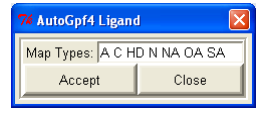
\includegraphics{autogrid4.PNG}
	\end{figure}
	\item Simpan berkas receptor dalam format *.gpf
\end{itemize}

\noindent \textbf{Menghitung atomic affinity maps} \\
Pemetaan yang sudah dilakukan pada receptor dan menghasilkan berkas receptor dalam format *.gpf harus dipetakan untuk setiap berkas ligand. Proses pemetaan ini dilakukan dengan cara menghitung atomic affinity maps pada berkas receptor dengan menggunakan aplikasi autogrid4. Tahapan ini akan menghasilkan berkas pemetaan dalam format *.glg, *.map, *maps.xyz dan *.maps.fld. Untuk mendapatkan hasil tersebut dapat dijalankan \textit{script} berikut pada \textit{desktop} PC yang telah terpasang Autodock Tools : \\
\begin{lstlisting}[caption=\textit{Script} untuk menghitung atomic affinity maps][frame=single]
#!bin/csh
/path/to/autogrid4 -p receptor.gpf -l receptor.glg
\end{lstlisting}
%-----------------------------------------------------------------------------%



\noindent \textbf{Mempersiapkan Docking Parameter Files} \\
Menyiapkan docking parameter files untuk setiap ligand dibantu modul phyton dari Autodock Tools 1.5.2 yang bernama prepare\_dpf4.py. Docking parameter files ini berisi informasi terkait ligand seperti jumlah atom, koordinat
atom dan jumlah torsi aktif yang dimiliki yang sudah dipetakan ke dalam informasi pada receptor. Hasil dari tahapan ini adalah berkas docking parameter files dalam format *.dpf. Jalankan modul prepare\_dpf4.py dengan \textit{script} berikut ini
\begin{lstlisting}[caption=\textit{script} untuk mempersiapkan docking parameter file]
for f in M*.pdbqt;do
name=`basename $f .pdbqt`
echo $name
/path/to/pythonsh /path/to /prepare_dpf.py -l $f -d
/path/to/ligand_dict.py -l `basename $f` -r
receptor.pdbqt \
-p ga_num_evals=1750000 \
-p ga_pop_size=150 \
-p ga_run=20 \
-p rmstol=2.0
End
\end{lstlisting}

\addChapter{Lampiran C}
\chapter*{Lampiran C}

\textbf{Kode yang digunakan dalam menjalankan eksperimen Autodock Vina versi 1.1} \\
\begin{lstlisting}[caption=\textit{Script} yang digunakan pada \textit{desktop} PC host dimana Docker terpasang]
#!/bin/bash

FILES="/percobaan2/*.pdbqt"
COUNTER_FILE=1
COUNTER_CONTAINER=1
NAMA_CONTAINER="vina"
COUNT=1
JUMLAH_FILE=0
LIMIT_FILE=0
RESIDU_FILE=0
JUMLAH_CONTAINER=$1

#menghitung banyaknya file yang dicopy kedalam container
let JUMLAH_FILE=`ls -1 /percobaan2/ | wc -l`
let LIMIT_FILE=$JUMLAH_FILE/$JUMLAH_CONTAINER
let RESIDU_FILE=$JUMLAH_FILE%$JUMLAH_CONTAINER
if [ $RESIDU_FILE -eq 0 ]
then 
let LIMIT_FILE=LIMIT_FILE+0
else
let LIMIT_FILE=LIMIT_FILE+1
fi

#main method
for f in $FILES
do 
if [ $COUNTER_FILE -eq 1 ]
then 
echo "Membuat container" $NAMA_CONTAINER$COUNTER_CONTAINER
docker run -i -t --name $NAMA_CONTAINER$COUNTER_CONTAINER -d agungputrap/riset_docker:latest
CONTAINER_ID=`docker inspect -f '{{.Id}}' $NAMA_CONTAINER$COUNTER_CONTAINER`
echo "ini nomor container = " $CONTAINER_ID
cp /3LP1O.pdbqt /var/lib/docker/aufs/diff/$CONTAINER_ID/3LP1O.pdbqt
cp /conf.txt /var/lib/docker/aufs/diff/$CONTAINER_ID/conf.txt
echo "mengcopy file "$COUNTER_FILE " ke container " $NAMA_CONTAINER$COUNTER_CONTAINER
cp $f /var/lib/docker/aufs/diff/$CONTAINER_ID/`basename $f`
echo "file dicopy " $COUNT
let COUNT=COUNT+1
let COUNTER_FILE=COUNTER_FILE+1
elif [ $COUNT -eq $JUMLAH_FILE ]
then 
echo "harusnya nilai terakhir "$COUNT
echo "mengcopy file terakhir ke container "$NAMA_CONTAINER$COUNTER_CONTAINER
cp $f /var/lib/docker/aufs/diff/$CONTAINER_ID/`basename $f`
cp /running_vina /var/lib/docker/aufs/diff/$CONTAINER_ID/running_vina
docker exec -d $NAMA_CONTAINER$COUNTER_CONTAINER chmod u+x /running_vina
docker exec -d $NAMA_CONTAINER$COUNTER_CONTAINER ./running_vina
elif [ $COUNTER_FILE -lt $LIMIT_FILE ]
then 
echo "mengcopy file "$COUNTER_FILE" ke container "$NAMA_CONTAINER$COUNTER_CONTAINER
cp $f /var/lib/docker/aufs/diff/$CONTAINER_ID/`basename $f`
echo "file dicopy " $COUNT
let COUNT=COUNT+1
let COUNTER_FILE=COUNTER_FILE+1
#case paling terakhir dijalanin
#	elif [ $COUNT -eq $JUMLAH_FILE ]
#	then 
#		echo "harusnya nilai terakhir "$COUNT
#		echo "mengcopy file terakhir ke container"$NAMA_CONTAINER$COUNTER_CONTAINER
#		cp $f /var/lib/docker/aufs/diff/$CONTAINER_ID/`basename $f`
#		cp /running_vina /var/lib/docker/aufs/$CONTAINER_ID/running_vina
#		docker exec -d $NAMA_CONTAINER$COUNTER_CONTAINER chmod u+x /running_vina
#		docker exec -d $NAMA_CONTAINER$COUNTER_CONTAINER ./running_vina
else
#mengcopy file terakhir dalam suatu container dan menjalankan script dalam container
echo "mengcopy file "$COUNTER_FILE" ke container "$NAMA_CONTAINER$COUNTER_CONTAINER
cp $f /var/lib/docker/aufs/diff/$CONTAINER_ID/`basename $f`
echo "file dicopy "$COUNT
let COUNT=COUNT+1
cp /running_vina /var/lib/docker/aufs/diff/$CONTAINER_ID/running_vina
docker exec -d $NAMA_CONTAINER$COUNTER_CONTAINER chmod u+x /running_vina
docker exec -d $NAMA_CONTAINER$COUNTER_CONTAINER ./running_vina
let COUNTER_FILE=1
let COUNTER_CONTAINER=COUNTER_CONTAINER+1
fi
done

\end{lstlisting}

\begin{lstlisting}[caption=\textit{Script} yang digunakan untuk menjalankan aplikasi Autodock Vina dalam container]
#!/bin/bash
FILES="/*.pdbqt"
echo "Waktu mulai " >> logvina.txt
date >> logvina.txt
for f in $FILES
do
./autodockvina/bin/vina --config conf.txt --ligand `basename $f`
done
echo "Waktu selesai " >> logvina.txt
date >> logvina.txt

\end{lstlisting}
\begin{lstlisting}[caption=\textit{Script} yang digunakan untuk mengambil hasil dari menjalankan aplikasi Autodock Vina pada container]
#!/bin/bash
COUNTER_CONTAINER=1
COUNTER=0
NAMA_CONTAINER="vina"
FILES="/var/lib/docker/aufs/diff/"
JUMLAH_FILE=0
let JUMLAH_FILE=`ls -1 /percobaan2/ | wc -l`
while [ $COUNTER -lt $JUMLAH_FILE ];
do
CONTAINER_ID=`docker inspect -f '{{.Id}}' $NAMA_CONTAINER$COUNTER_CONTAINER`
FILEX="$FILES$CONTAINER_ID/*_out.pdbqt"
echo $FILEX
for f in $FILEX
do
docker cp $NAMA_CONTAINER$COUNTER_CONTAINER:`basename $f` /hasilvina/
let COUNTER=COUNTER+1
done
let COUNTER_CONTAINER=COUNTER_CONTAINER+1
done

\end{lstlisting}

\begin{lstlisting}[caption=\textit{Script} yang digunakan untuk mengambil log dari masing - masing container]
#!/bin/bash
COUNTER_CONTAINER=1
COUNTER=0
NAMA_CONTAINER="vina"
FILES="/var/lib/docker/aufs/diff/"
JUMLAH_FILE=$1
while [ $COUNTER -lt $JUMLAH_FILE ];
do
CONTAINER_ID=`docker inspect -f '{{.Id}}' $NAMA_CONTAINER$COUNTER_CONTAINER`
FILEX="$FILES$CONTAINER_ID/logvina*"
echo $FILEX
for f in $FILEX
do
docker cp $NAMA_CONTAINER$COUNTER_CONTAINER:`basename $f` /logvina/$NAMA_CONTAINER$COUNTER_CONTAINER/
let COUNTER=COUNTER+1
done
let COUNTER_CONTAINER=COUNTER_CONTAINER+1
done

\end{lstlisting}

\addChapter{Lampiran D}
\chapter*{Lampiran D}
\textbf{Kode yang digunakan dalam menjalankan eksperimen Autodock versi 4.2} \\

\begin{lstlisting}[caption=\textit{Script} yang digunakan pada \textit{desktop} PC untuk membuat container dan menjalankan container]
#!/bin/bash

FILES="/percobaan2/*.pdbqt"
COUNTER_FILE=1
COUNTER_CONTAINER=1
NAMA_CONTAINER="dock"
COUNT=1
JUMLAH_FILE=0
LIMIT_FILE=0
RESIDU_FILE=0
JUMLAH_CONTAINER=$1

#menghitung banyaknya file yang dicopy kedalam container
let JUMLAH_FILE=`ls -1 /percobaan2/ | wc -l`
let LIMIT_FILE=$JUMLAH_FILE/$JUMLAH_CONTAINER
let RESIDU_FILE=$JUMLAH_FILE%$JUMLAH_CONTAINER
if [ $RESIDU_FILE -eq 0 ]
then 
let LIMIT_FILE=LIMIT_FILE+0
else
let LIMIT_FILE=LIMIT_FILE+1
fi

#main method
for f in $FILES
do 
if [ $COUNTER_FILE -eq 1 ]
then 
echo "Membuat container" $NAMA_CONTAINER$COUNTER_CONTAINER
docker run -i -t --name $NAMA_CONTAINER$COUNTER_CONTAINER -d agungputrap/riset_docker:latest
CONTAINER_ID=`docker inspect -f '{{.Id}}' $NAMA_CONTAINER$COUNTER_CONTAINER`
echo "ini nomor container = " $CONTAINER_ID
cp /3LP1O* /var/lib/docker/aufs/diff/$CONTAINER_ID/
#		memproses ligand menjadi .dpf dan mengcopy ke dalam container beserta ligand
echo "memproses file "$COUNTER_FILE
./home/agungpp/MGLTools-1.5.6/MGLToolsPckgs/AutoDockTools/Utilities24/prepare_dpf4.py -l $f -r /3LP1O.pdbqt 
NAMA=`basename $f .pdbqt`
OUTPUT_PREPARE=$NAMA"_3LP1O.dpf"
cp /$OUTPUT_PREPARE /var/lib/docker/aufs/diff/$CONTAINER_ID/$OUTPUT_PREPARE
echo "mengcopy file "$COUNTER_FILE " ke container " $NAMA_CONTAINER$COUNTER_CONTAINER
cp $f /var/lib/docker/aufs/diff/$CONTAINER_ID/`basename $f`
echo "file dicopy " $COUNT
let COUNT=COUNT+1
let COUNTER_FILE=COUNTER_FILE+1
elif [ $COUNT -eq $JUMLAH_FILE ]
then 
echo "harusnya nilai terakhir "$COUNT
echo "memproses file terakhir "
./home/agungpp/MGLTools-1.5.6/MGLToolsPckgs/AutoDockTools/Utilities24/prepare_dpf4.py -l $f -r /3LP1O.pdbqt
NAMA=`basename $f .pdbqt`
OUTPUT_PREPARE=$NAMA"_3LP1O.dpf"
cp /$OUTPUT_PREPARE /var/lib/docker/aufs/diff/$CONTAINER_ID/$OUTPUT_PREPARE
echo "mengcopy file " $COUNTER_FILE " ke container " $NAMA_CONTAINER$COUNTER_$CONTAINER
cp $f /var/lib/docker/aufs/diff/$CONTAINER_ID/`basename $f`
cp /running_dock /var/lib/docker/aufs/diff/$CONTAINER_ID/running_dock
docker exec -d $NAMA_CONTAINER$COUNTER_CONTAINER chmod u+x /running_dock
docker exec -d $NAMA_CONTAINER$COUNTER_CONTAINER ./running_dock
elif [ $COUNTER_FILE -lt $LIMIT_FILE ]
then 
echo "memproses file " $COUNTER_FILE
./home/agungpp/MGLTools-1.5.6/MGLToolsPckgs/AutoDockTools/Utilities24/prepare_dpf4.py -l $f -r /3LP1O.pdbqt
NAMA=`basename $f .pdbqt`
OUTPUT_PREPARE=$NAMA"_3LP1O.dpf"
cp /$OUTPUT_PREPARE /var/lib/docker/aufs/diff/$CONTAINER_ID/$OUTPUT_PREPARE
echo "mengcopy file "$COUNTER_FILE" ke container "$NAMA_CONTAINER$COUNTER_CONTAINER
cp $f /var/lib/docker/aufs/diff/$CONTAINER_ID/`basename $f`
echo "file dicopy " $COUNT
let COUNT=COUNT+1
let COUNTER_FILE=COUNTER_FILE+1
#case paling terakhir dijalanin
#	elif [ $COUNT -eq $JUMLAH_FILE ]
#	then 
#		echo "harusnya nilai terakhir "$COUNT
#		echo "mengcopy file terakhir ke container"$NAMA_CONTAINER$COUNTER_CONTAINER
#		cp $f /var/lib/docker/aufs/diff/$CONTAINER_ID/`basename $f`
#		cp /running_vina /var/lib/docker/aufs/$CONTAINER_ID/running_vina
#		docker exec -d $NAMA_CONTAINER$COUNTER_CONTAINER chmod u+x /running_vina
#		docker exec -d $NAMA_CONTAINER$COUNTER_CONTAINER ./running_vina
else
#mengcopy file terakhir dalam suatu container dan menjalankan script dalam container
echo "memproses file " $COUNTER_FILE
./home/agungpp/MGLTools-1.5.6/MGLToolsPckgs/AutoDockTools/Utilities24/prepare_dpf4.py -l $f -r /3LP1O.pdbqt
NAMA=`basename $f .pdbqt`
OUTPUT_PREPARE=$NAMA"_3LP1O.dpf"
cp /$OUTPUT_PREPARE /var/lib/docker/aufs/diff/$CONTAINER_ID/$OUTPUT_PREPARE
echo "mengcopy file "$COUNTER_FILE" ke container "$NAMA_CONTAINER$COUNTER_CONTAINER
cp $f /var/lib/docker/aufs/diff/$CONTAINER_ID/`basename $f`
echo "file dicopy "$COUNT
let COUNT=COUNT+1
cp /running_dock /var/lib/docker/aufs/diff/$CONTAINER_ID/running_dock
docker exec -d $NAMA_CONTAINER$COUNTER_CONTAINER chmod u+x /running_dock
docker exec -d $NAMA_CONTAINER$COUNTER_CONTAINER ./running_dock
let COUNTER_FILE=1
let COUNTER_CONTAINER=COUNTER_CONTAINER+1
fi
done

\end{lstlisting}

\begin{lstlisting}[caption=\textit{Script} yang dijalankan pada masing - masing container]
#!/bin/bash
FILES="/*_3LP1O.dpf"
echo "Waktu mulai " >> logdock.txt
date >> logdock.txt
for f in $FILES
do
./autodock/autodock4 -p $f -l `basename $f .dpf`.dlg
done
echo "Waktu selesai " >> logdock.txt
date >> logdock.txt

\end{lstlisting}

\begin{lstlisting}[caption=\textit{Script} yang digunakan untuk mengambil hasil dari menjalankan aplikasi Autodock dari masing - masing container]
#!/bin/bash
COUNTER_CONTAINER=1
COUNTER=0
NAMA_CONTAINER="dock"
FILES="/var/lib/docker/aufs/diff/"
JUMLAH_FILE=0
let JUMLAH_FILE=`ls -1 /percobaan2/ | wc -l`
while [ $COUNTER -lt $JUMLAH_FILE ];
do
CONTAINER_ID=`docker inspect -f '{{.Id}}' $NAMA_CONTAINER$COUNTER_CONTAINER`
FILEX="$FILES$CONTAINER_ID/*.dlg"
echo $FILEX
for f in $FILEX
do
docker cp $NAMA_CONTAINER$COUNTER_CONTAINER:`basename $f` /hasildock/
let COUNTER=COUNTER+1
done
let COUNTER_CONTAINER=COUNTER_CONTAINER+1
done

\end{lstlisting}
\begin{lstlisting}[caption=\textit{Script} yang digunakan untuk mengambil log dari masing - masing container]
#!/bin/bash
COUNTER_CONTAINER=1
COUNTER=0
NAMA_CONTAINER="dock"
FILES="/var/lib/docker/aufs/diff/"
JUMLAH_FILE=$1
while [ $COUNTER -lt $JUMLAH_FILE ];
do
CONTAINER_ID=`docker inspect -f '{{.Id}}' $NAMA_CONTAINER$COUNTER_CONTAINER`
FILEX="$FILES$CONTAINER_ID/logdock*"
echo $FILEX
for f in $FILEX
do
docker cp $NAMA_CONTAINER$COUNTER_CONTAINER:`basename $f` /logdock/$NAMA_CONTAINER$COUNTER_CONTAINER/
let COUNTER=COUNTER+1
done
let COUNTER_CONTAINER=COUNTER_CONTAINER+1
done

\end{lstlisting}
\end{appendix}

\end{document}